\chapter{Results}
\label{ch:7}

% **************************** Define Graphics Path **************************
\ifpdf
    \graphicspath{{Chapter7/Figs/Raster/}{Chapter7/Figs/PDF/}{Chapter7/Figs/}}
\else
    \graphicspath{{Chapter7/Figs/Vector/}{Chapter7/Figs/}}
\fi


%********************************** % First Section  *************************************
\section{Likelihood Model}  %Section - 1.1 
\label{sec:results_likelihood}
The likelihood model is defined for each analysis category of \nb and \nj.

\subsection{Hadronic Signal Region}

Let $n^i$ be the observed number of events 
following full selection in the $i^{th}$ of $N$ bins of \HT. The likelihood is 
constructed as:

\begin{equation}
L_{hadronic} = \prod_i \text{Pois}(n^i | b^i + s^i),
\end{equation}

where $b^i$ and $s^i$ represent the expected number of background events from SM 
processes and the expected number of signal events in the bin $i$. Pois is 
the Poisson distribution:

\begin{equation}
f(k;\lambda) = \frac{1}{k!}\lambda^k e^{-\lambda}.
\end{equation}


\subsection{Electroweak Background Contribution}
The background is considered to be entirely EWK in origin ($b^i = \text{EWK}^i$), as QCD
is made negligible, so can be deconstructed using the relative fraction
of \zinv events, \fzinv as:

\begin{equation}
\text{Z}_{inv}^i = \fzinv \times \text{EWK}^i,
\label{eq:ewk_frac_z}
\end{equation}
\begin{equation}
\text{ttW}^i = (1-\fzinv) \times \text{EWK}^i,
\label{eq:ewk_frac_ttw}
\end{equation}

where $\text{EWK}^i$ is number of expected events from the total EWK background,
$\text{Z}_{\text{inv}}^i$ is the number of expected events from the \zinv 
contribution and $\text{ttW}^i$ is the number of expect events from the W boson 
production and top quark decay contribution, all in the $i^{th}$ bin. The variable 
\fzinv is allowed to float between 0 and 1.

EWK backgrounds are predicted using sideband control samples and transfer 
factors (chapter~\ref{ch:6}). Let $n_{\gamma}^i$, $n_{\mu}^i$ and $n_{\mu\mu}^i$ be 
the observed event counts in the \gj, \mj and \mmj control samples, 
respectively, with corresponding yields in MC: \mcp, \mcm, \mcmm. These are
further seperated into seperate contributions from \zinv,
\mczinv, and \text{ttW}, \mcttw. Transfer
factors are defined as the inverse as those of the analysis:

\begin{equation}
r_{\gamma}^i = \frac{\mcp}{\mczinv};\;\;\;
r_{\mu\mu}^i = \frac{\mcmm}{\mczinv};\;\;\;
r_{\mu}^i = \frac{\mcm}{\mcttw},
\end{equation}

and so likelihoods are written as:

\begin{equation}
L_{\gamma} = \prod_i \text{Pois}(n_{\gamma}^i | \rhopz \cdot r^i_{\gamma} \cdot Z^i_{\text{inv}}),
\label{eq:lterm_pho}
\end{equation}
\begin{equation}
L_{\mu\mu} = \prod_i \text{Pois}(n_{\mu\mu}^i | \rhommz \cdot r^i_{\mu\mu} \cdot Z^i_{\text{inv}}),
\label{eq:lterm_mumu}
\end{equation}
\begin{equation}
L_{\mu} = \prod_i \text{Pois}(n_{\mu}^i | \rhomw \cdot r^i_{\mu} \cdot ttW^i + s_{\mu}^i).
\label{eq:lterm_mu}
\end{equation}

Both equations~\ref{eq:lterm_pho} and \ref{eq:lterm_mumu} are used to estimate the 
maximum likelihood value for $Z^i_{\text{inv}}$, alongside equation~\ref{eq:lterm_mu} 
for $ttW^i$, all considered simulataneously through the relationships defined in
equations~\ref{eq:ewk_frac_z} and \ref{eq:ewk_frac_ttw}.

The terms \rhopz, \rhommz and \rhomw are correction factors accomodating the
systematic uncertainties associated with the control sample based background 
predictions. The relative uncertainties are derived in
section~\ref{sec:closure_tests} and represented by the terms \sigmapz, \sigmammz
and \sigmamw, their 
values summarised in table~\ref{tab:syst_values}. Systematics enter the total
likelihood as:

\begin{equation}
L_{\gamma\text{ syst.}} = \prod_j \text{Logn}(1.0 | \rhopz, \sigmapz),
\end{equation}
\begin{equation}
L_{\mu\mu\text{ syst.}} = \prod_j \text{Logn}(1.0 | \rhommz, \sigmammz),
\end{equation}
\begin{equation}
L_{\mu\text{ syst.}} = \prod_j \text{Logn}(1.0 | \rhomw, \sigmamw),
\end{equation}

where Logn is the log-normal distribution (as recommended by \cite{cousins-log-normal}):

\begin{equation}
\text{Logn}(x|\mu, \sigma) = \frac{1}{x\sqrt{2\pi}\text{ln}k} exp \Bigg(-\frac{\text{ln}^2 \big(\frac{x}{\mu}\big)}{2\text{ln}^2k}\Bigg); k = 1+\sigma
\end{equation}

These terms are combined as:

\begin{equation}
L_{EWK\text{ syst.}} = L_{\gamma\text{ syst.}} \times L_{\mu\mu\text{ syst.}} \times L_{\mu\text{ syst.}}.
\end{equation}

For $\nb \geq 2$ categories, the \mj control sample is used to predict \zinv and
\ttw combined, giving:

\begin{equation}
{r'}^i_{\mu} = \frac{\mcm}{MC^i_{\ttbar + W + Z_{\text{inv}}}};
\end{equation}

\begin{equation}
L_{\mu} = \prod_i \text{Pois}(n_{\mu}^i | \rhomw \cdot {r'}_{\mu}^i \cdot {EWK}^i + s_{\mu}^i).
\end{equation}

Terms corresponding to the \mmj and \gj samples are subsequently dropped.

\subsection{Signal Contribution}

Let $x$ be the cross section of the signal model under test, which can be varied
according to a multiplicative factor $f$ (a.k.a. the ``mu-factor''), and $l$ be 
the luminosity of the relevant collected data sample. $\epsilon^i_{had}$ and
$\epsilon^i_{\mu}$ are the signal acceptances of the hadronic and muon 
selections, respectively, for the given signal model. Finally, let $\delta$ be 
the relative systematic uncertainty on that signal acceptance, and $\rho_{sig}$ 
be the corrective factor to the signal yield floated to accomodate this uncertainty. 
Therefore the yield of signal events for the hadronic sample, $s^i$, and the 
yield of signal in the muon sample (i.e. ``signal contamination''), $s^i_{\mu}$,
can be written as:

\begin{equation}
s^i = f\rho_{sig}xl\epsilon_{had}
\end{equation}
\begin{equation}
s^i_{\mu} = f\rho_{sig}xl\epsilon_{\mu}
\end{equation}

Furthermore, the signal systematic contribution to the likelihood is included as
the term:

\begin{equation}
L_{signal} = \text{Logn}(1.0 | \rho_{sig}, \delta)
\end{equation}

\subsection{Total Likelihood}

For a given analysis category $k$ (\nb, \nj), the total likelihood is 
constructed as:

\begin{equation}
L^k_{total} = L^k_{hadronic} \times L^k_{\mu} \times L^k_{\gamma} \times L^k_{\mu\mu} 
\times L^k_{\text{EWK syst.}}
\label{eq:total_likelihood}
\end{equation}

The number of nuisance paramters varies between different analysis categories, 
dependent on the number of \HT bins and control samples, summarised in
table~\ref{tab:nuisance_param_summary}.

\begin{table}[ht!]
  \caption{Summary of nuisance parameters.}
  \label{tab:nuisance_param_summary}
  \centering
  \footnotesize
  \begin{tabular}{ lll }
    \hline
    \hline
    Description                             & Categories    & Nuisance Parameters \\ [1.0ex]
    \hline
    \multirow{2}{*}{11 \HT bins, ($\mu, \mu\mu, \gamma$)}    & \multirow{2}{*}{\njlow/\njhigh, \nb = 0, 1}&
    $\{EWK^i, \fzinv\}_{i=0}^{10}, \{ \rhopz \}_{i=3}^{6},$\\
    && $\{ \rhommz, \rhomw \}_{i=0}^{6}$  \\
    8 \HT bins, ($\mu$)                     & \njlow/\njhigh, \nb = 2, 3, >4    & $\{EWK^i, \fzinv\}_{i=0}^{
    8}, \{\rhomwz \}_{i=0}^{6}$  \\
    3 \HT bins, ($\mu$)                     & \njlow/\njhigh, \nb = 2, 3, >4    & $\{EWK^i\}_{i=0}^{3},
    \{\rhomwz \}_{i=0}$\\
    \hline
    \hline
  \end{tabular}
\end{table}

When considering signal an additional term is introduced:

\begin{equation}
L = L_{signal} \times \prod_k L^k_{total}
\label{eq:total_likelihood_wsignal}
\end{equation}

% \subsection{Notes on syst modelling}
% lognormal instead of gaussian PDF - these are used for systematics modelling.

% see:
% \verb!http://www.physics.ucla.edu/~cousins/stats/cousins_lognormal_prior.pdf!

% if you had a parameter with mean of 0.3 and variance of 0.1, you could have a 
% distro which would give you negative values of your PDF, if you used gaussian. 
% therefore we use lognormal.

% The lognormal distribution has three variables as input. $Logn(x|\rho, \sigma)$

% \begin{description}
% \item[$\sigma$ parameter]\hfill \\ this is similar to the width, if it were a gaussian 
% distribution. It is essentially the derived systematic error as taken from the 
% closure tests (I think...!). The smaller the value, the more the $\rho$ 
% parameters may need to be pulled in order to make the fit.
% \item[$\rho$ parameter] \hfill \\ the mean of the syst error. this is a parameter
% (nuisance?) which is allowed to float in the fit. It essentially represents how 
% much you have to pull on your systematics in order for the observations to match
% the background predictions. If it's pulled a lot (many sigma away from 1.) then 
% your observations really don't fit your predictions, or you've really 
% underestimated your systematics! Large deviations from 1 (in terms of the
% $\sigma$ parameter) indicate an unhealthy fit...
% \end{description}



%********************************** % Second Section  *************************************
\section{Fit Results}  %Section - 1.2
\label{sec:results_fit}
The likelihood model described in section~\ref{sec:results_likelihood} is used
to relate the observations in the signal and control samples, accomodate the
calculated background systematic uncertainties, and allow for the presence of
any potential signal. In order to test the compatibility with a Standard
Model only hypotheis, signal contribution is set to zero and the likilhood is
maximized over all parameter using RooFit \cite{roofit} and \MINUIT
\cite{James:1975dr}, for each analysis category of \nb and \nj.

Uncertainties are determined by performing a number of pseudo-experiments for
each (\nb, \nj) category and \HT bin, with the fit yields being put into a
histogram, appropriate quantiles taken, using their difference from the maximum 
likelihood (ML) value taken as the uncertainty value.

Two different procedures are used to determine fits to observations, as described
in the following sections.

\subsection{Fit without Signal region}
An ``a priori'' fit is made by considering only yields from the control samples,
and not data observations in the hadronic signal region. The results of this fit
are shown in figures~REF and summarised in tabular form in
table~\ref{tab:ensemble-summary-priori}.

\begin{landscape}
\begin{center}
\begin{table}[h!]
  \caption{Summary of the ``a posteriori'' fit.}
  \label{tab:ensemble-summary-posteriori}
  \centering
  \scriptsize
  \begin{tabular}{ llllllllllllll }
    \hline
    \hline
    \multicolumn{2}{c}{} & \multicolumn{11}{c}{\HT (GeV)}                                                                                                                                                                                                                                            \\ 
    \nj                & \nb      &        & 200--275              & 275--325             & 325--375             & 375--475             & 475--575             & 575--675             & 675--775             & 775--875             & 875--975             & 975--1075           & 1075--$\infty$      \\ 
    \hline
    2--3                 & $0$      & SM   & $13235^{+119}_{-101}$ & $5417^{+73}_{-62}$   & $3562^{+69}_{-48}$   & $2482^{+38}_{-40}$   & $689^{+15}_{-13}$    & $231^{+13}_{-10}$    & $72.2^{+5.2}_{-4.0}$ & $28.1^{+3.2}_{-3.0}$ & $11.2^{+1.4}_{-1.6}$ & $6.0^{+1.1}_{-0.9}$ & $3.7^{+0.9}_{-0.7}$ \\ 
    2--3                 & $0$      & Data & $13090$               & $5331$               & $3354$               & $2326$               & $671$                & $206$                & $76$                 & $29$                 & $10$                 & $9$                 & $2$                 \\\\
    2--3                 & $1$      & SM   & $1743^{+32}_{-32}$    & $843^{+23}_{-26}$    & $580^{+23}_{-18}$    & $413^{+16}_{-14}$    & $102^{+5}_{-5}$      & $27.0^{+2.8}_{-2.9}$ & $9.1^{+1.2}_{-1.2}$  & $3.3^{+0.7}_{-0.7}$  & $2.3^{+0.7}_{-0.6}$  & $0.3^{+0.2}_{-0.1}$ & $0.2^{+0.1}_{-0.1}$ \\ 
    2--3                 & $1$      & Data & $1733$                & $833.0$              & $527.0$              & $356.0$              & $90.0$               & $31.0$               & $6.0$                & $4.0$                & $1.0$                & $0.0$               & $1.0$               \\\\
    2--3                 & $2$      & SM   & $176^{+8}_{-6}$       & $115^{+6}_{-6}$      & $104^{+6}_{-5}$      & $68.1^{+4.7}_{-4.7}$ & $15.2^{+1.6}_{-1.5}$ & $3.3^{+0.5}_{-0.6}$  & $1.1^{+0.3}_{-0.3}$  & $0.2^{+0.1}_{-0.1}$  & $0.1^{+0.0}_{-0.0}$  & \multicolumn{2}{c}{}                      \\ 
    2--3                 & $2$      & Data & $172$                 & $116$                & $101$                & $55$                 & $16$                 & $9$                  & $0$                  & $0$                  & $0$                  & \multicolumn{2}{c}{}                      \\ \\
    $\geq 4$             & $0$      & SM   & $104^{+6}_{-8}$       & $567^{+21}_{-20}$    & $454^{+20}_{-19}$    & $397^{+14}_{-14}$    & $250^{+11}_{-10}$    & $134^{+10}_{-8}$     & $55.5^{+4.4}_{-4.1}$ & $19.2^{+2.5}_{-2.1}$ & $9.8^{+1.6}_{-1.4}$  & $4.6^{+1.0}_{-1.0}$ & $4.2^{+1.0}_{-0.9}$ \\ 
    $\geq 4$             & $0$      & Data & $99$                  & $568$                & $408$                & $336$                & $211$                & $117$                & $38$                 & $13$                 & $9$                  & $4$                 & $6$                 \\\\
    $\geq 4$             & $1$      & SM   & $39.4^{+3.0}_{-3.0}$  & $216^{+9}_{-9}$      & $238^{+13}_{-14}$    & $179^{+9}_{-10}$     & $104^{+6}_{-6}$      & $36.4^{+3.5}_{-3.3}$ & $14.2^{+1.8}_{-1.8}$ & $8.6^{+1.5}_{-1.4}$  & $3.9^{+0.9}_{-0.8}$  & $1.1^{+0.4}_{-0.3}$ & $1.2^{+0.4}_{-0.4}$ \\ 
    $\geq 4$             & $1$      & Data & $38$                  & $195$                & $210$                & $159$                & $83$                 & $33$                 & $7$                  & $10$                 & $4$                  & $1$                 & $1$                 \\\\
    $\geq 4$             & $2$      & SM   & $13.3^{+1.0}_{-1.0}$  & $77.1^{+4.4}_{-4.4}$ & $95.5^{+7.7}_{-6.7}$ & $77.4^{+5.7}_{-5.9}$ & $48.2^{+3.7}_{-3.7}$ & $18.4^{+3.1}_{-2.4}$ & $6.2^{+1.0}_{-0.9}$  & $1.7^{+0.4}_{-0.4}$  & $1.8^{+0.4}_{-0.3}$  & \multicolumn{2}{c}{}                      \\ 
    $\geq 4$             & $2$      & Data & $16$                  & $81$                 & $88$                 & $64$                 & $43$                 & $14$                 & $5$                  & $1$                  & $1$                  & \multicolumn{2}{c}{}                      \\\\ 
    $\geq 4$             & $3$      & SM   & $1.0^{+0.2}_{-0.2}$   & $8.2^{+0.8}_{-0.8}$  & $10.9^{+1.6}_{-1.5}$ & $8.2^{+1.1}_{-1.1}$  & $5.8^{+1.0}_{-0.8}$  & $2.2^{+0.6}_{-0.5}$  & $0.9^{+0.3}_{-0.2}$  & $0.2^{+0.1}_{-0.1}$  & $0.2^{+0.1}_{-0.1}$  & \multicolumn{2}{c}{}                      \\ 
    $\geq 4$             & $3$      & Data & $0$                   & $7$                  & $5$                  & $5$                  & $6$                  & $1$                  & $1$                  & $0$                  & $0$                  & \multicolumn{2}{c}{}                      \\\\ 
    $\geq 4$             & $\geq 4$ & SM   & $0.0^{+0.0}_{-0.0}$   & $0.1^{+0.1}_{-0.1}$  & $0.5^{+0.3}_{-0.3}$  & $0.9^{+0.3}_{-0.3}$  & \multicolumn{7}{l}{}                                                                                                                                         \\ 
    $\geq 4$             & $\geq 4$ & Data & $0$                   & $0$                  & $0$                  & $2$                  & \multicolumn{7}{l}{}                                                                                                                                         \\ 
    \hline
    \hline
  \end{tabular}
\end{table}
\end{center}
\end{landscape}

\subsection{Fit with Signal region}
An ``a posteriori'' fit is made by considering every region, including the
hadronic signal region's observation in data, and is shown in
figures~REF and
summarised in table~\ref{tab:ensemble-summary-posteriori}.

\begin{landscape}
\begin{center}
\begin{table}[h!]
  \caption{Summary of the ``a priori'' fit.}
  \label{tab:ensemble-summary-priori}
  \centering
  \scriptsize
  \begin{tabular}{ llllllllllllll }
    \hline
    \hline
    \multicolumn{2}{c}{} & \multicolumn{11}{c}{\HT (GeV)}                                                                                                                                                                                                                                              \\ 
    \nj                & \nb      &        & 200--275              & 275--325             & 325--375              & 375--475             & 475--575              & 575--675             & 675--775             & 775--875             & 875--975             & 975--1075           & 1075--$\infty$      \\ 
    \hline
    2--3                 & $0$      & SM   & $12391^{+368}_{-325}$ & $5566^{+325}_{-188}$ & $3424^{+205}_{-149}$  & $2473^{+131}_{-96}$  & $684^{+38}_{-34}$     & $231^{+18}_{-19}$    & $69.8^{+6.1}_{-6.6}$ & $27.9^{+3.9}_{-3.2}$ & $11.0^{+2.1}_{-1.8}$ & $5.4^{+0.8}_{-1.0}$ & $3.7^{+0.9}_{-0.8}$ \\ 
    2--3                 & $0$      & Data & $13090$               & $5331$               & $3354$                & $2326$               & $671$                 & $206$                & $76$                 & $29$                 & $10$                 & $9$                 & $2$                 \\\\
    2--3                 & $1$      & SM   & $1626^{+60}_{-47}$    & $862^{+48}_{-41}$    & $548^{+29}_{-35}$     & $413^{+28}_{-23}$    & $103^{+8}_{-7}$       & $26.6^{+3.1}_{-3.2}$ & $9.5^{+1.2}_{-1.6}$  & $3.1^{+0.9}_{-0.8}$  & $2.6^{+0.9}_{-0.8}$  & $0.4^{+0.2}_{-0.2}$ & $0.2^{+0.1}_{-0.1}$ \\ 
    2--3                 & $1$      & Data & $1733$                & $833.0$              & $527.0$               & $356.0$              & $90.0$                & $31.0$               & $6.0$                & $4.0$                & $1.0$                & $0.0$               & $1.0$               \\\\
    2--3                 & $2$      & SM   & $177^{+9}_{-7}$       & $113^{+7}_{-7}$      & $97.3^{+6.3}_{-6.6}$  & $66.0^{+6.3}_{-5.8}$ & $14.6^{+1.7}_{-1.4}$  & $2.9^{+0.5}_{-0.5}$  & $1.1^{+0.2}_{-0.3}$  & $0.2^{+0.1}_{-0.1}$  & $0.1^{+0.1}_{-0.0}$  & \multicolumn{2}{c}{}                      \\ 
    2--3                 & $2$      & Data & $172$                 & $116$                & $101$                 & $55$                 & $16$                  & $9$                  & $0$                  & $0$                  & $0$                  & \multicolumn{2}{c}{}                      \\ \\
    $\geq 4$             & $0$      & SM   & $106^{+10}_{-10}$     & $520^{+32}_{-34}$    & $448^{+39}_{-54}$     & $369^{+31}_{-25}$    & $224^{+17}_{-15}$     & $109^{+14}_{-13}$    & $46.8^{+5.8}_{-6.1}$ & $19.2^{+2.8}_{-2.7}$ & $9.2^{+1.7}_{-1.7}$  & $3.7^{+1.1}_{-0.9}$ & $3.2^{+0.7}_{-0.7}$ \\ 
    $\geq 4$             & $0$      & Data & $99$                  & $568$                & $408$                 & $336$                & $211$                 & $117$                & $38$                 & $13$                 & $9$                  & $4$                 & $6$                 \\\\
    $\geq 4$             & $1$      & SM   & $39.8^{+3.2}_{-3.5}$  & $223^{+14}_{-12}$    & $211^{+25}_{-23}$     & $171^{+18}_{-15}$    & $98.7^{+10.1}_{-9.1}$ & $35.5^{+6.0}_{-5.1}$ & $14.8^{+2.2}_{-2.2}$ & $6.8^{+1.5}_{-1.2}$  & $3.2^{+0.9}_{-0.9}$  & $1.1^{+0.5}_{-0.4}$ & $1.2^{+0.4}_{-0.4}$ \\ 
    $\geq 4$             & $1$      & Data & $38$                  & $195$                & $210$                 & $159$                & $83$                  & $33$                 & $7$                  & $10$                 & $4$                  & $1$                 & $1$                 \\\\
    $\geq 4$             & $2$      & SM   & $13.0^{+1.0}_{-0.9}$  & $75.5^{+4.8}_{-4.8}$ & $96.1^{+11.4}_{-9.4}$ & $69.5^{+7.2}_{-8.3}$ & $43.9^{+4.8}_{-5.7}$  & $16.1^{+3.7}_{-2.7}$ & $5.2^{+1.2}_{-0.9}$  & $1.7^{+0.3}_{-0.4}$  & $1.9^{+0.5}_{-0.4}$  & \multicolumn{2}{c}{}                      \\ 
    $\geq 4$             & $2$      & Data & $16$                  & $81$                 & $88$                  & $64$                 & $43$                  & $14$                 & $5$                  & $1$                  & $1$                  & \multicolumn{2}{c}{}                      \\\\ 
    $\geq 4$             & $3$      & SM   & $1.0^{+0.2}_{-0.2}$   & $8.1^{+0.8}_{-0.8}$  & $11.7^{+1.9}_{-1.6}$  & $8.0^{+1.4}_{-1.2}$  & $5.3^{+1.2}_{-0.8}$   & $2.3^{+0.6}_{-0.5}$  & $0.8^{+0.2}_{-0.2}$  & $0.2^{+0.1}_{-0.1}$  & $0.2^{+0.1}_{-0.1}$  & \multicolumn{2}{c}{}                      \\ 
    $\geq 4$             & $3$      & Data & $0$                   & $7$                  & $5$                   & $5$                  & $6$                   & $1$                  & $1$                  & $0$                  & $0$                  & \multicolumn{2}{c}{}                      \\\\ 
    $\geq 4$             & $\geq 4$ & SM   & $0.0^{+0.0}_{-0.0}$   & $0.1^{+0.1}_{-0.1}$  & $0.6^{+0.3}_{-0.3}$   & $0.7^{+0.3}_{-0.3}$  & \multicolumn{7}{l}{}                                                                                                                                          \\ 
    $\geq 4$             & $\geq 4$ & Data & $0$                   & $0$                  & $0$                   & $2$                  & \multicolumn{7}{l}{}                                                                                                                                         \\ 
    \hline
    \hline
  \end{tabular}
\end{table}
\end{center}
\end{landscape}

\subsection{Pulls and p-values}
no signal! background only
\emph{what does each plot mean?}


%%%%%%%%%%%%%%%%%%%%%%%%%%%%%%%%%%%
% GREEN BAND PLOTS
%%%%%%%%%%%%%%%%%%%%%%%%%%%%%%%%%%%

\clearpage
\begin{figure}[h!]
  \centering
  \begin{subfigure}[b]{0.48\textwidth}
    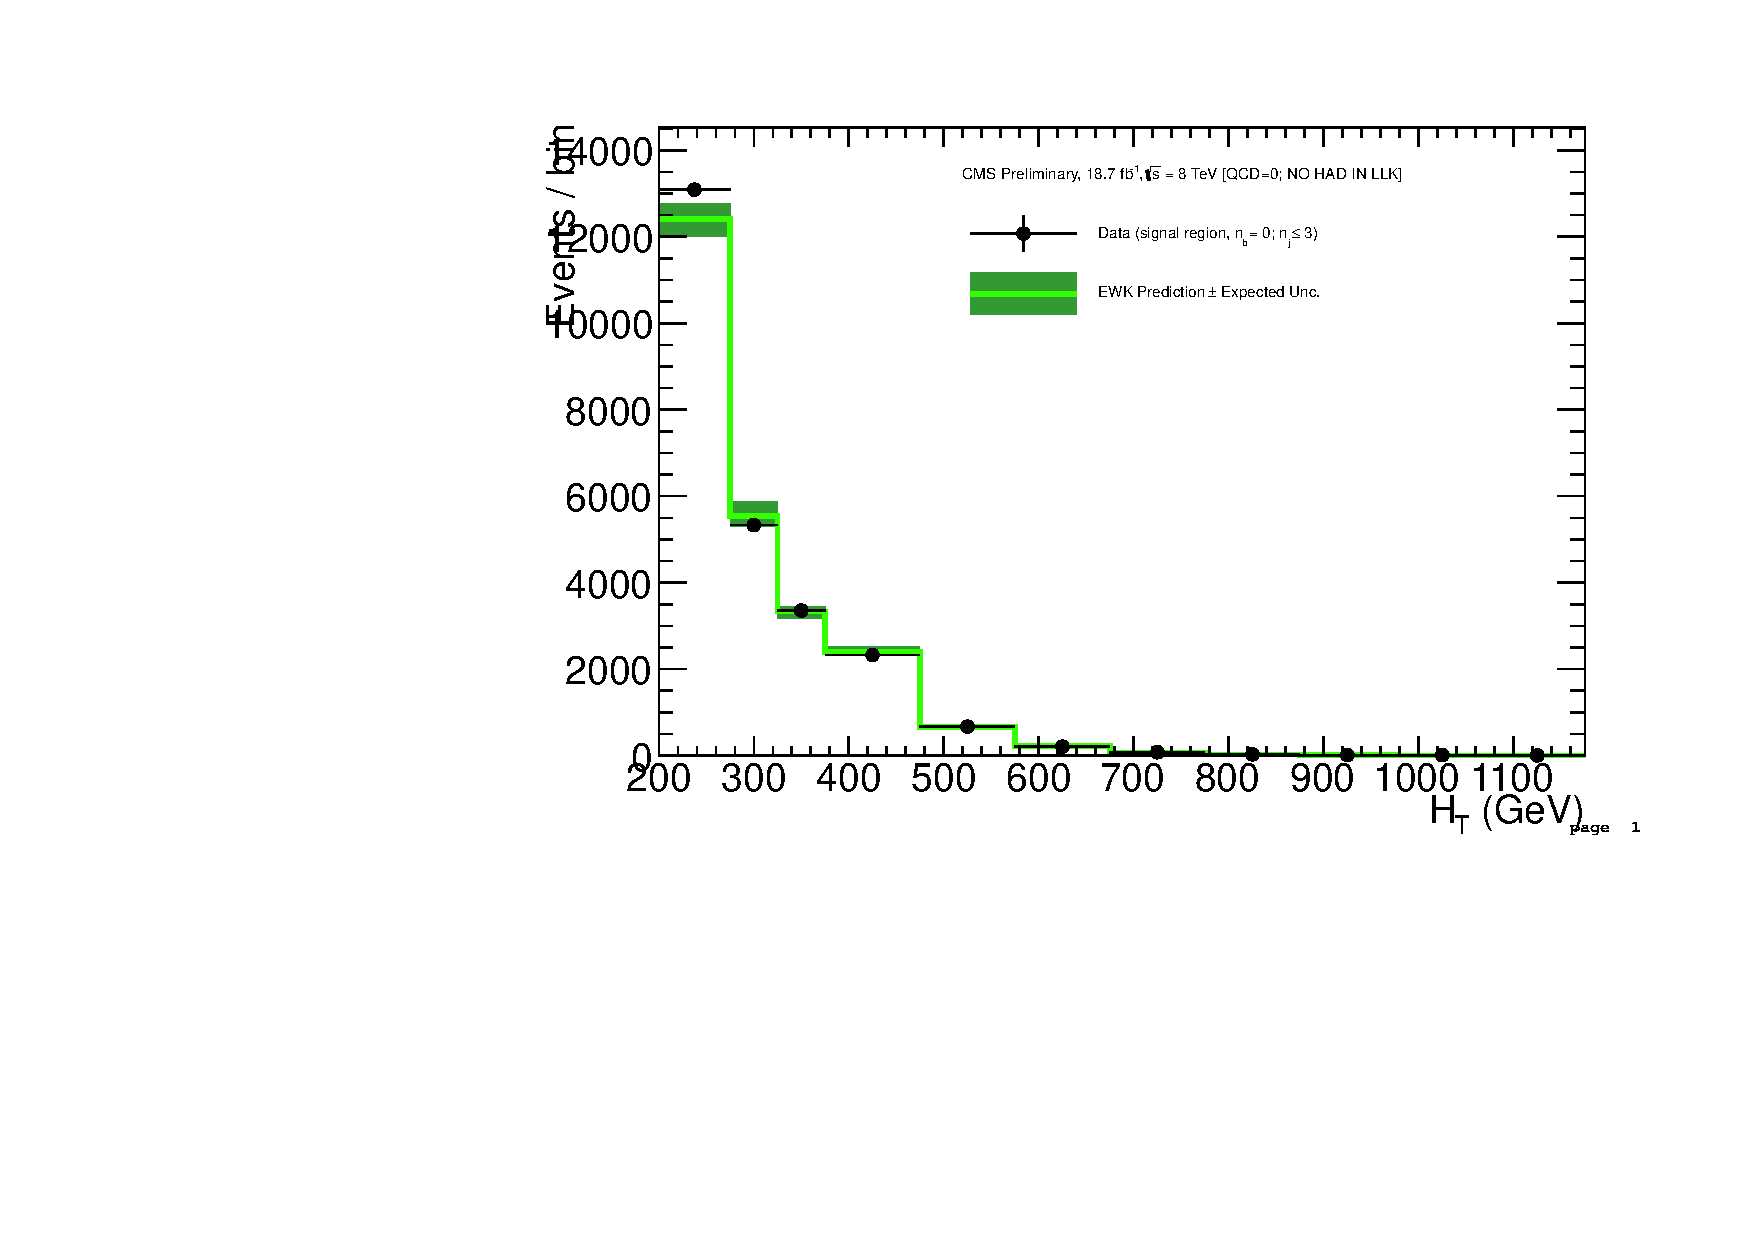
\includegraphics[width=\textwidth,page=1]
    {Figs/results/v0/greenBand/bestFit_2012dev_RQcdZero_fZinvAll_0b_le3j-12p_smOnly}
    \caption{Hadronic sample (linear scale)}
  \end{subfigure}
  \begin{subfigure}[b]{0.48\textwidth}
    \includegraphics[width=\textwidth,page=2]
    {Figs/results/v0/greenBand/bestFit_2012dev_RQcdZero_fZinvAll_0b_le3j-12p_smOnly}
    \caption{Hadronic sample (logarithmic scale)}
  \end{subfigure}
  \begin{subfigure}[b]{0.48\textwidth}
    \includegraphics[width=\textwidth,page=4]
    {Figs/results/v0/greenBand/bestFit_2012dev_RQcdZero_fZinvAll_0b_le3j-12p_smOnly}
    \caption{\mj sample}
  \end{subfigure}
  \begin{subfigure}[b]{0.48\textwidth}
    \includegraphics[width=\textwidth,page=8]
    {Figs/results/v0/greenBand/bestFit_2012dev_RQcdZero_fZinvAll_0b_le3j-12p_smOnly}
    \caption{\mmj sample}
  \end{subfigure}\\
  \begin{subfigure}[b]{0.48\textwidth}
    \includegraphics[width=\textwidth,page=6]
    {Figs/results/v0/greenBand/bestFit_2012dev_RQcdZero_fZinvAll_0b_le3j-12p_smOnly}
    \caption{\gj sample}
  \end{subfigure}
  \caption{\njlow, $\nb = 0$}
  \label{fig:green_fits_0b_le3j}
\end{figure}

\clearpage
\begin{figure}[h!]
  \centering
  \begin{subfigure}[b]{0.48\textwidth}
    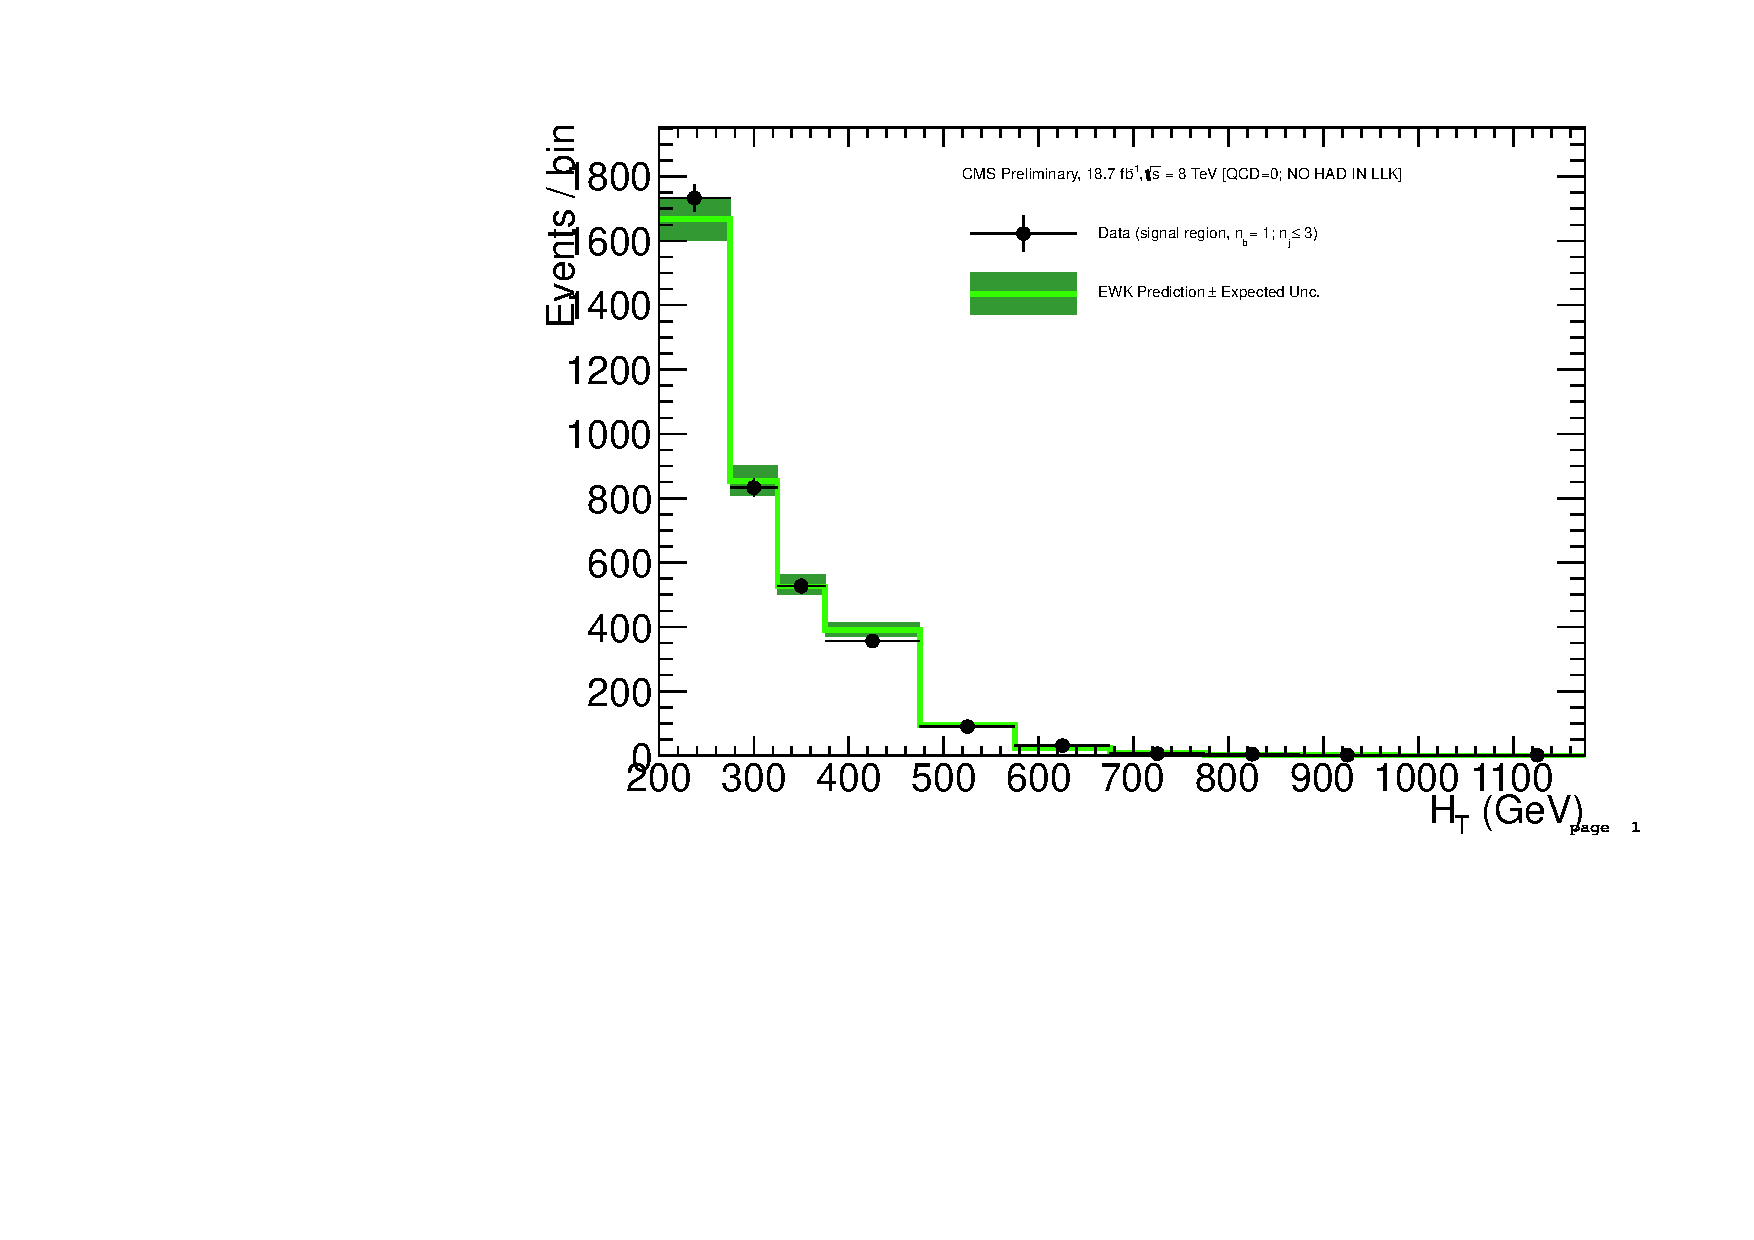
\includegraphics[width=\textwidth,page=1]
    {Figs/results/v0/greenBand/bestFit_2012dev_RQcdZero_fZinvAll_1b_le3j-12p_smOnly}
    \caption{Hadronic sample (linear scale)}
  \end{subfigure}
  \begin{subfigure}[b]{0.48\textwidth}
    \includegraphics[width=\textwidth,page=2]
    {Figs/results/v0/greenBand/bestFit_2012dev_RQcdZero_fZinvAll_1b_le3j-12p_smOnly}
    \caption{Hadronic sample (logarithmic scale)}
  \end{subfigure}
  \begin{subfigure}[b]{0.48\textwidth}
    \includegraphics[width=\textwidth,page=4]
    {Figs/results/v0/greenBand/bestFit_2012dev_RQcdZero_fZinvAll_1b_le3j-12p_smOnly}
    \caption{\mj sample}
  \end{subfigure}
  \begin{subfigure}[b]{0.48\textwidth}
    \includegraphics[width=\textwidth,page=8]
    {Figs/results/v0/greenBand/bestFit_2012dev_RQcdZero_fZinvAll_1b_le3j-12p_smOnly}
    \caption{\mmj sample}
  \end{subfigure}\\
  \begin{subfigure}[b]{0.48\textwidth}
    \includegraphics[width=\textwidth,page=6]
    {Figs/results/v0/greenBand/bestFit_2012dev_RQcdZero_fZinvAll_1b_le3j-12p_smOnly}
    \caption{\gj sample}
  \end{subfigure}
  \caption{\njlow, $\nb = 1$}
  \label{fig:green_fits_1b_le3j}
\end{figure}

\clearpage
\begin{figure}[h!]
  \centering
  \begin{subfigure}[b]{0.48\textwidth}
    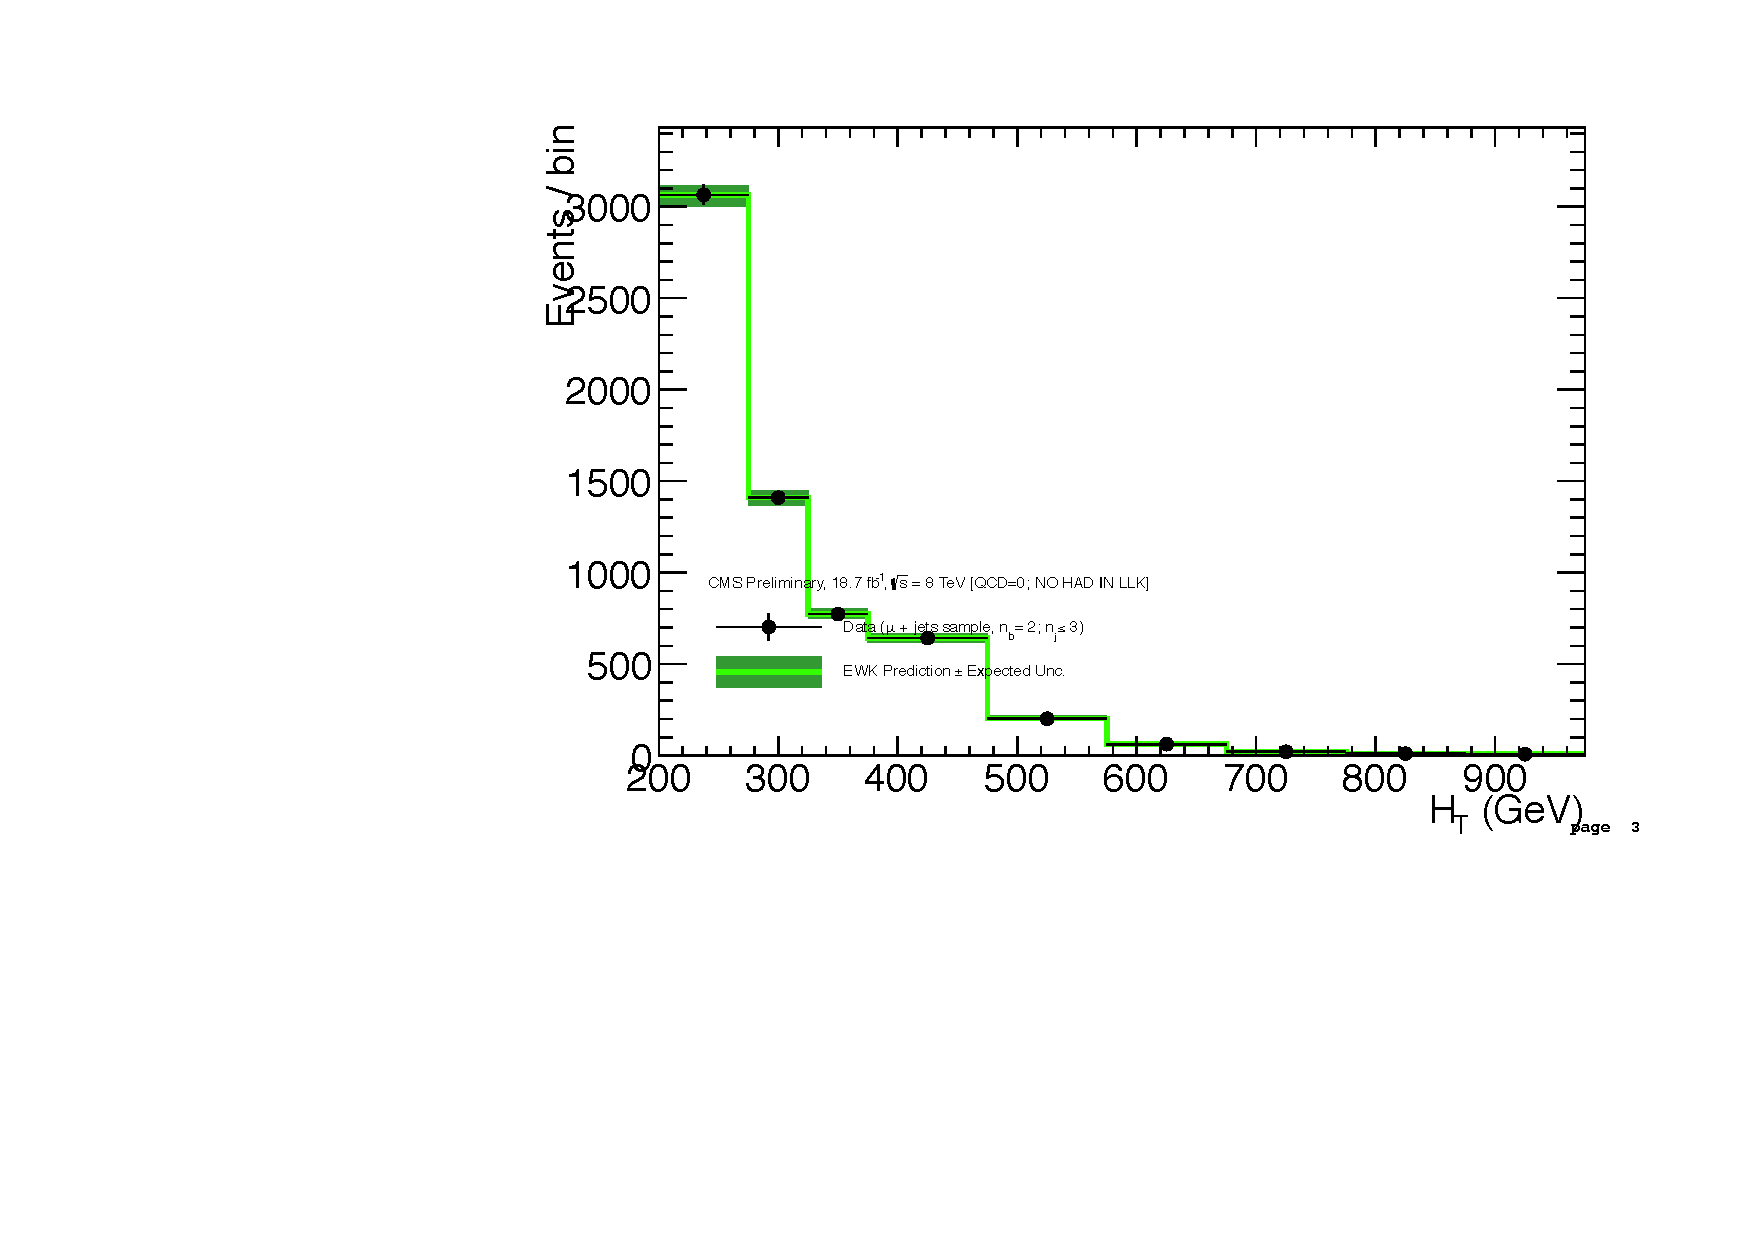
\includegraphics[width=\textwidth,page=1]
    {Figs/results/v0/greenBand/bestFit_2012dev_RQcdZero_fZinvAll_2b_le3j-1_smOnly}
    \caption{Hadronic sample (linear scale)}
  \end{subfigure}
  \begin{subfigure}[b]{0.48\textwidth}
    \includegraphics[width=\textwidth,page=2]
    {Figs/results/v0/greenBand/bestFit_2012dev_RQcdZero_fZinvAll_2b_le3j-1_smOnly}
    \caption{Hadronic sample (logarithmic scale)}
  \end{subfigure}
  \begin{subfigure}[b]{0.48\textwidth}
    \includegraphics[width=\textwidth,page=4]
    {Figs/results/v0/greenBand/bestFit_2012dev_RQcdZero_fZinvAll_2b_le3j-1_smOnly}
    \caption{\mj sample}
  \end{subfigure}
  \caption{\njlow, $\nb = 2$}
  \label{fig:green_fits_2b_le3j}
\end{figure}

\clearpage
\begin{figure}[h!]
  \centering
  \begin{subfigure}[b]{0.48\textwidth}
    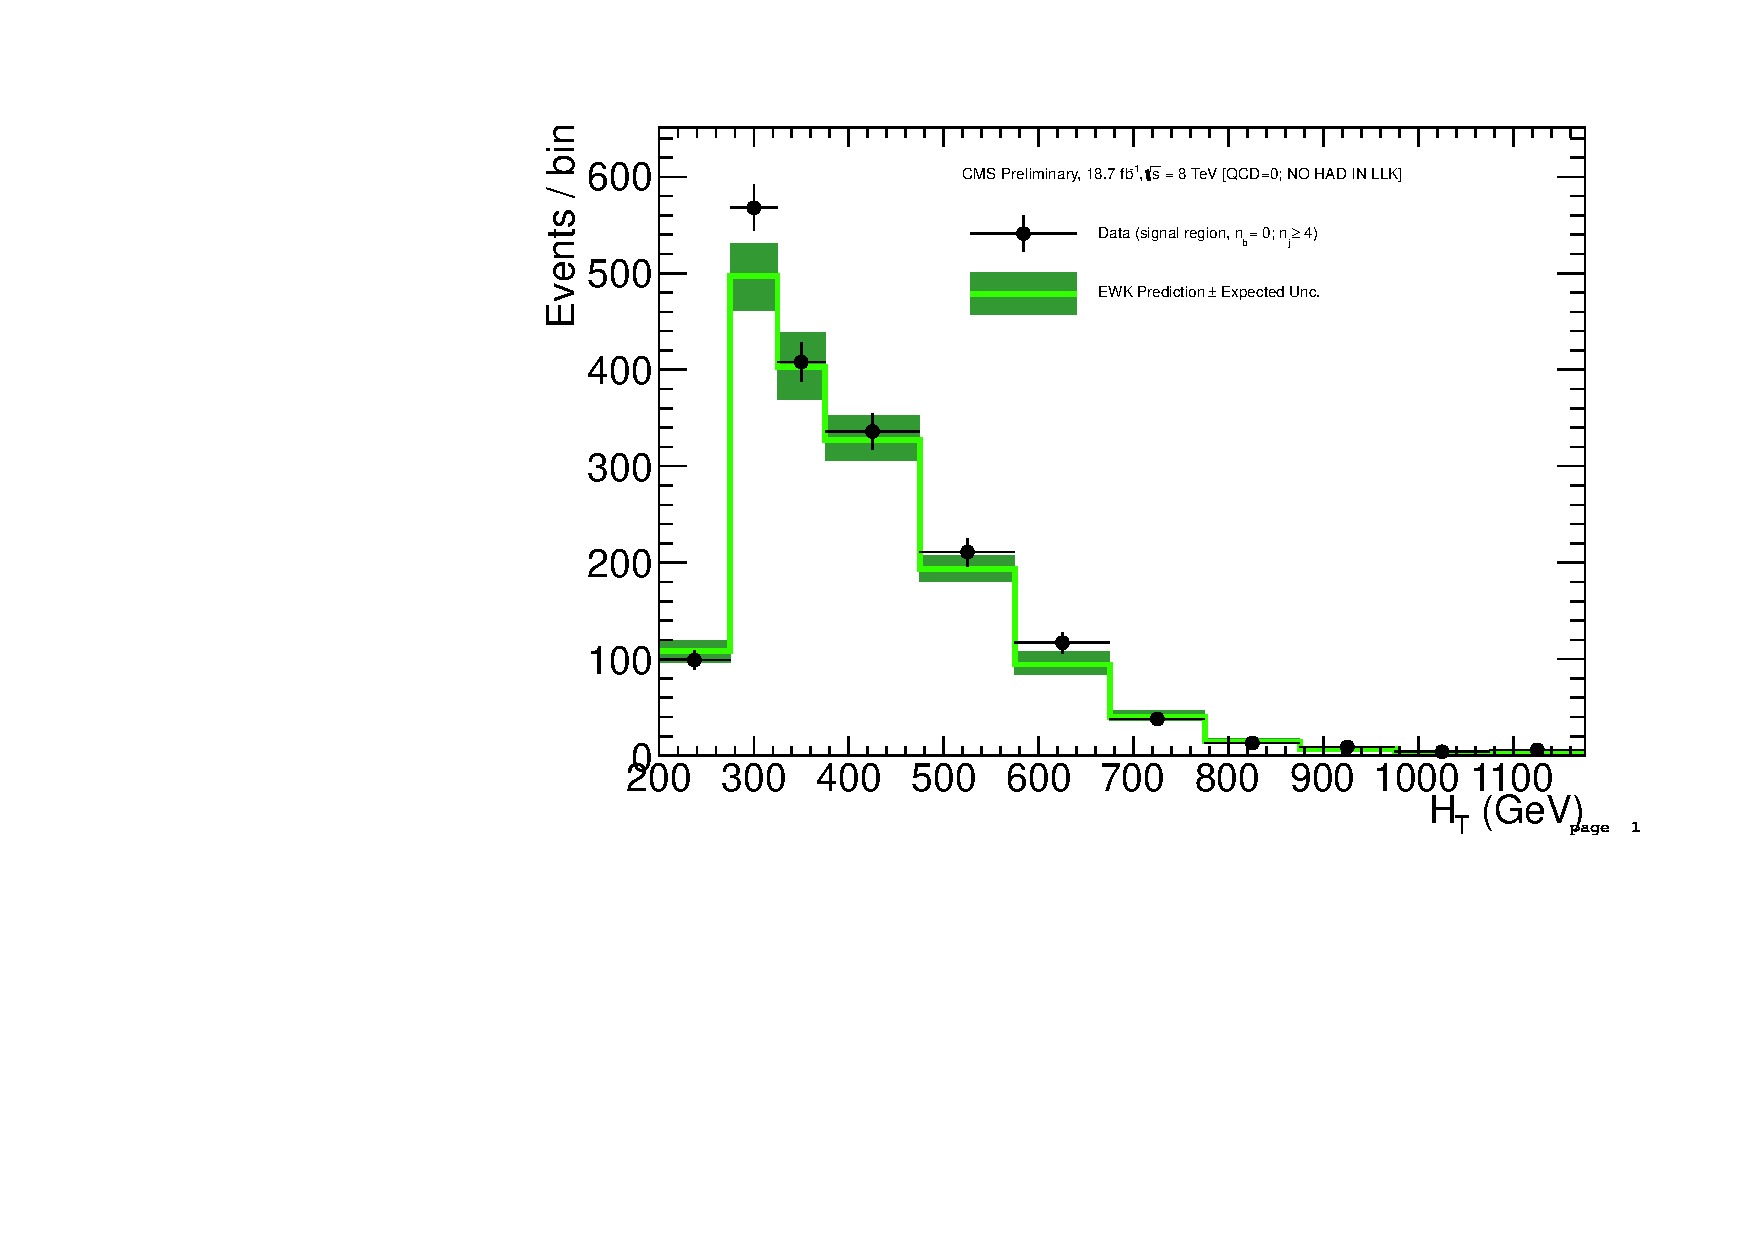
\includegraphics[width=\textwidth,page=1]
    {Figs/results/v0/greenBand/bestFit_2012dev_RQcdZero_fZinvAll_0b_ge4j-12p_smOnly}
    \caption{Hadronic sample (linear scale)}
  \end{subfigure}
  \begin{subfigure}[b]{0.48\textwidth}
    \includegraphics[width=\textwidth,page=2]
    {Figs/results/v0/greenBand/bestFit_2012dev_RQcdZero_fZinvAll_0b_ge4j-12p_smOnly}
    \caption{Hadronic sample (logarithmic scale)}
  \end{subfigure}
  \begin{subfigure}[b]{0.48\textwidth}
    \includegraphics[width=\textwidth,page=4]
    {Figs/results/v0/greenBand/bestFit_2012dev_RQcdZero_fZinvAll_0b_ge4j-12p_smOnly}
    \caption{\mj sample}
  \end{subfigure}
  \begin{subfigure}[b]{0.48\textwidth}
    \includegraphics[width=\textwidth,page=8]
    {Figs/results/v0/greenBand/bestFit_2012dev_RQcdZero_fZinvAll_0b_ge4j-12p_smOnly}
    \caption{\mmj sample}
  \end{subfigure}\\
  \begin{subfigure}[b]{0.48\textwidth}
    \includegraphics[width=\textwidth,page=6]
    {Figs/results/v0/greenBand/bestFit_2012dev_RQcdZero_fZinvAll_0b_ge4j-12p_smOnly}
    \caption{\gj sample}
  \end{subfigure}
  \caption{\njhigh, $\nb = 0$}
  \label{fig:green_fits_0b_ge4j}
\end{figure}

\clearpage
\begin{figure}[h!]
  \centering
  \begin{subfigure}[b]{0.48\textwidth}
    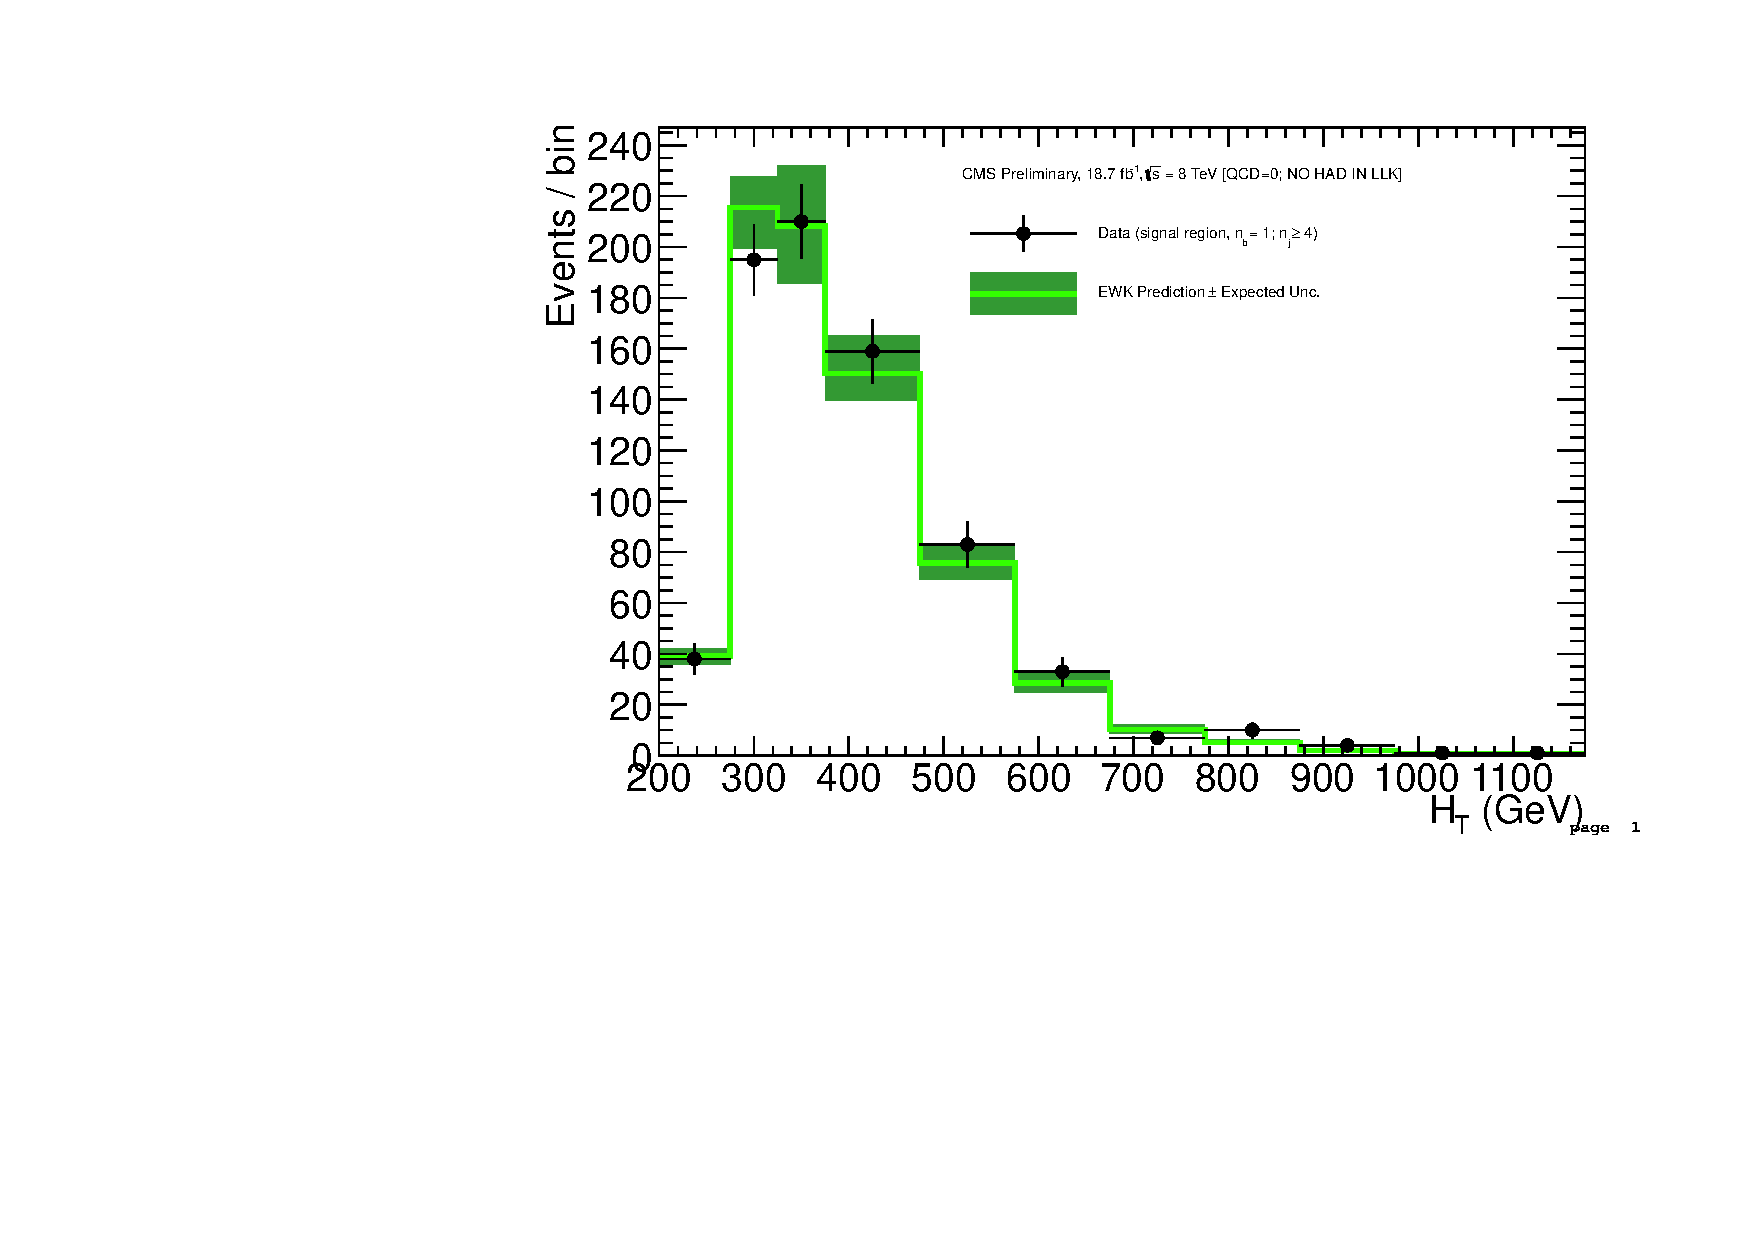
\includegraphics[width=\textwidth,page=1]
    {Figs/results/v0/greenBand/bestFit_2012dev_RQcdZero_fZinvAll_1b_ge4j-12p_smOnly}
    \caption{Hadronic sample (linear scale)}
  \end{subfigure}
  \begin{subfigure}[b]{0.48\textwidth}
    \includegraphics[width=\textwidth,page=2]
    {Figs/results/v0/greenBand/bestFit_2012dev_RQcdZero_fZinvAll_1b_ge4j-12p_smOnly}
    \caption{Hadronic sample (logarithmic scale)}
  \end{subfigure}
  \begin{subfigure}[b]{0.48\textwidth}
    \includegraphics[width=\textwidth,page=4]
    {Figs/results/v0/greenBand/bestFit_2012dev_RQcdZero_fZinvAll_1b_ge4j-12p_smOnly}
    \caption{\mj sample}
  \end{subfigure}
  \begin{subfigure}[b]{0.48\textwidth}
    \includegraphics[width=\textwidth,page=8]
    {Figs/results/v0/greenBand/bestFit_2012dev_RQcdZero_fZinvAll_1b_ge4j-12p_smOnly}
    \caption{\mmj sample}
  \end{subfigure}\\
  \begin{subfigure}[b]{0.48\textwidth}
    \includegraphics[width=\textwidth,page=6]
    {Figs/results/v0/greenBand/bestFit_2012dev_RQcdZero_fZinvAll_1b_ge4j-12p_smOnly}
    \caption{\gj sample}
  \end{subfigure}
  \caption{\njhigh, $\nb = 1$}
  \label{fig:green_fits_1b_ge4j}
\end{figure}

\clearpage
\begin{figure}[h!]
  \centering
  \begin{subfigure}[b]{0.48\textwidth}
    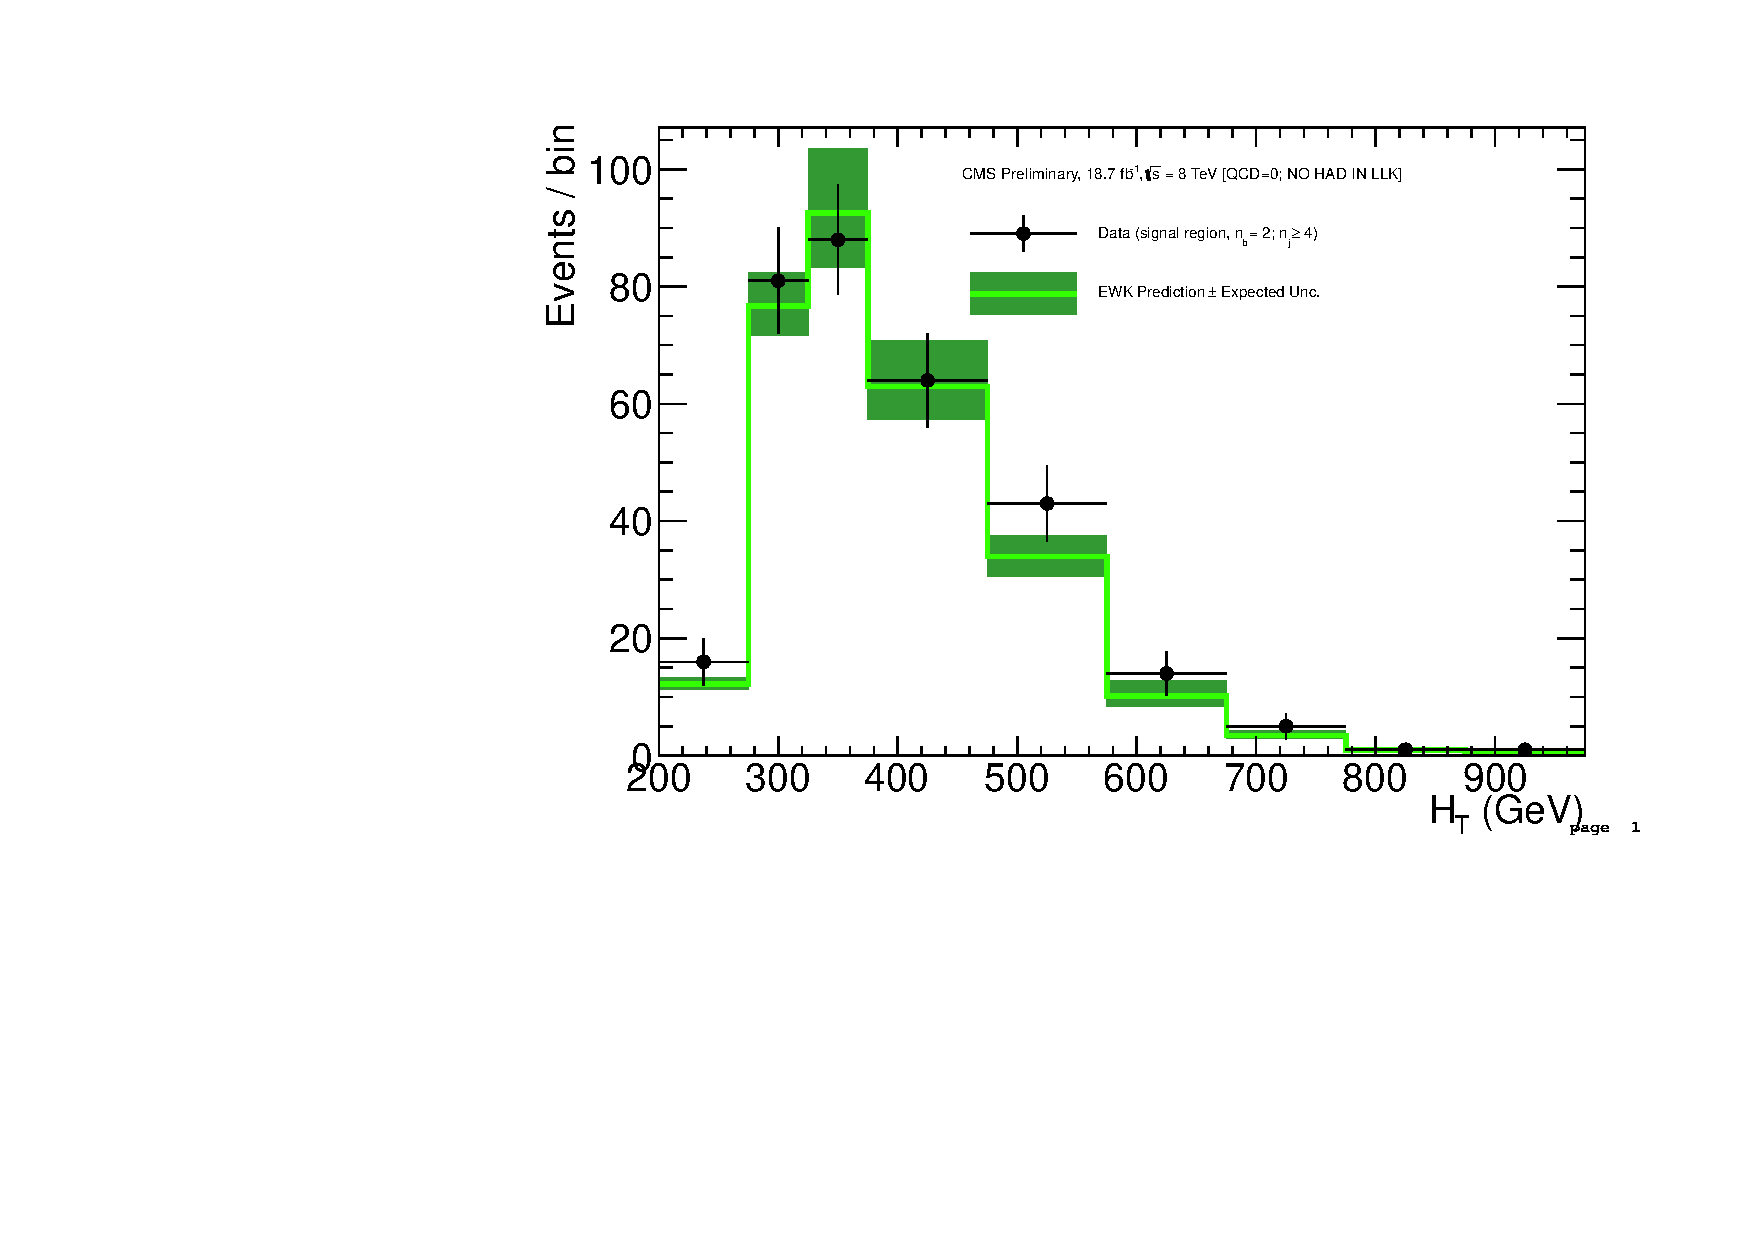
\includegraphics[width=\textwidth,page=1]
    {Figs/results/v0/greenBand/bestFit_2012dev_RQcdZero_fZinvAll_2b_ge4j-1_smOnly}
    \caption{Hadronic sample (linear scale)}
  \end{subfigure}
  \begin{subfigure}[b]{0.48\textwidth}
    \includegraphics[width=\textwidth,page=2]
    {Figs/results/v0/greenBand/bestFit_2012dev_RQcdZero_fZinvAll_2b_ge4j-1_smOnly}
    \caption{Hadronic sample (logarithmic scale)}
  \end{subfigure}
  \begin{subfigure}[b]{0.48\textwidth}
    \includegraphics[width=\textwidth,page=4]
    {Figs/results/v0/greenBand/bestFit_2012dev_RQcdZero_fZinvAll_2b_ge4j-1_smOnly}
    \caption{\mj sample}
  \end{subfigure}
  \caption{\njhigh, $\nb = 2$}
  \label{fig:green_fits_2b_ge4j}
\end{figure}


\clearpage
\begin{figure}[h!]
  \centering
  \begin{subfigure}[b]{0.48\textwidth}
    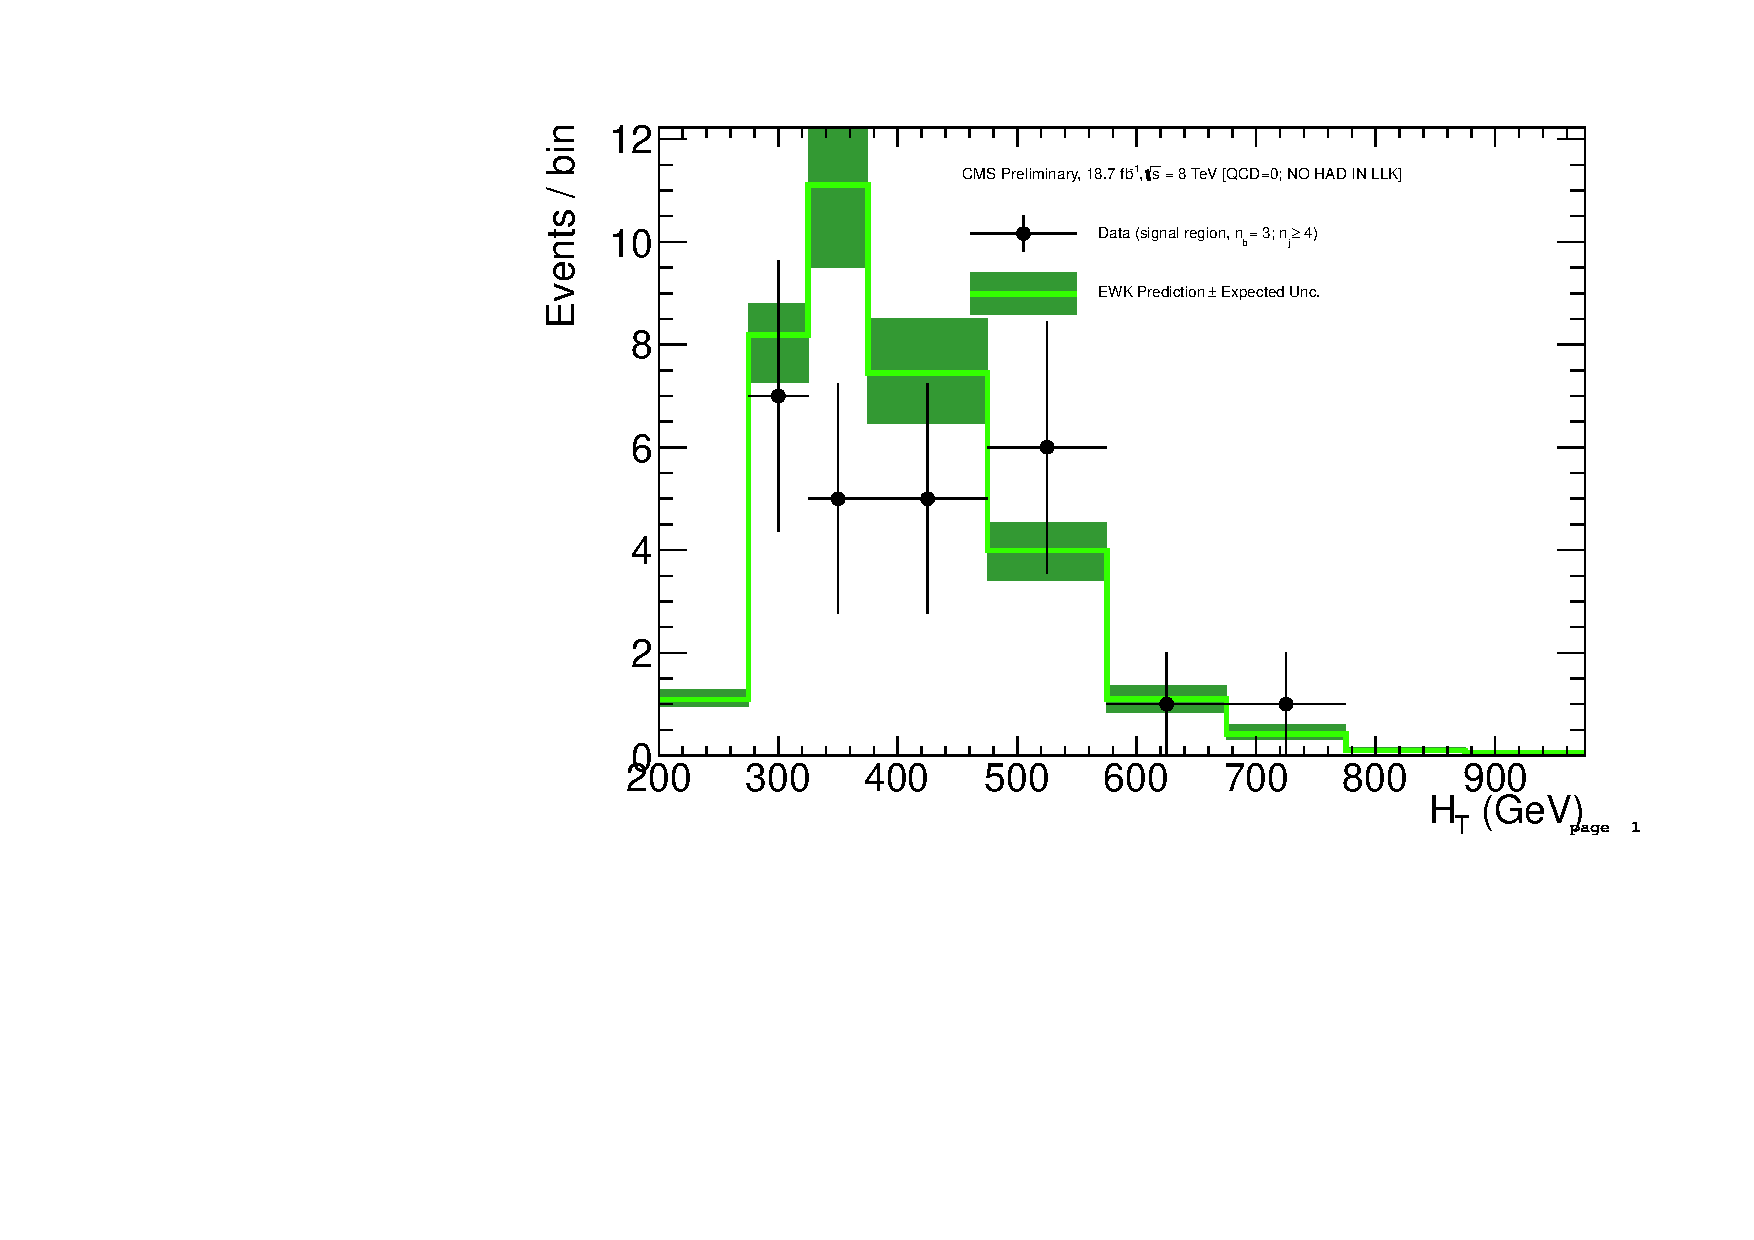
\includegraphics[width=\textwidth,page=1]
    {Figs/results/v0/greenBand/bestFit_2012dev_RQcdZero_fZinvAll_3b_ge4j-1_smOnly}
    \caption{Hadronic sample (linear scale)}
  \end{subfigure}
  \begin{subfigure}[b]{0.48\textwidth}
    \includegraphics[width=\textwidth,page=2]
    {Figs/results/v0/greenBand/bestFit_2012dev_RQcdZero_fZinvAll_3b_ge4j-1_smOnly}
    \caption{Hadronic sample (logarithmic scale)}
  \end{subfigure}
  \begin{subfigure}[b]{0.48\textwidth}
    \includegraphics[width=\textwidth,page=4]
    {Figs/results/v0/greenBand/bestFit_2012dev_RQcdZero_fZinvAll_3b_ge4j-1_smOnly}
    \caption{\mj sample}
  \end{subfigure}
  \caption{\njhigh, $\nb = 3$}
  \label{fig:green_fits_3b_ge4j}
\end{figure}

\clearpage
\begin{figure}[h!]
  \centering
  \begin{subfigure}[b]{0.48\textwidth}
    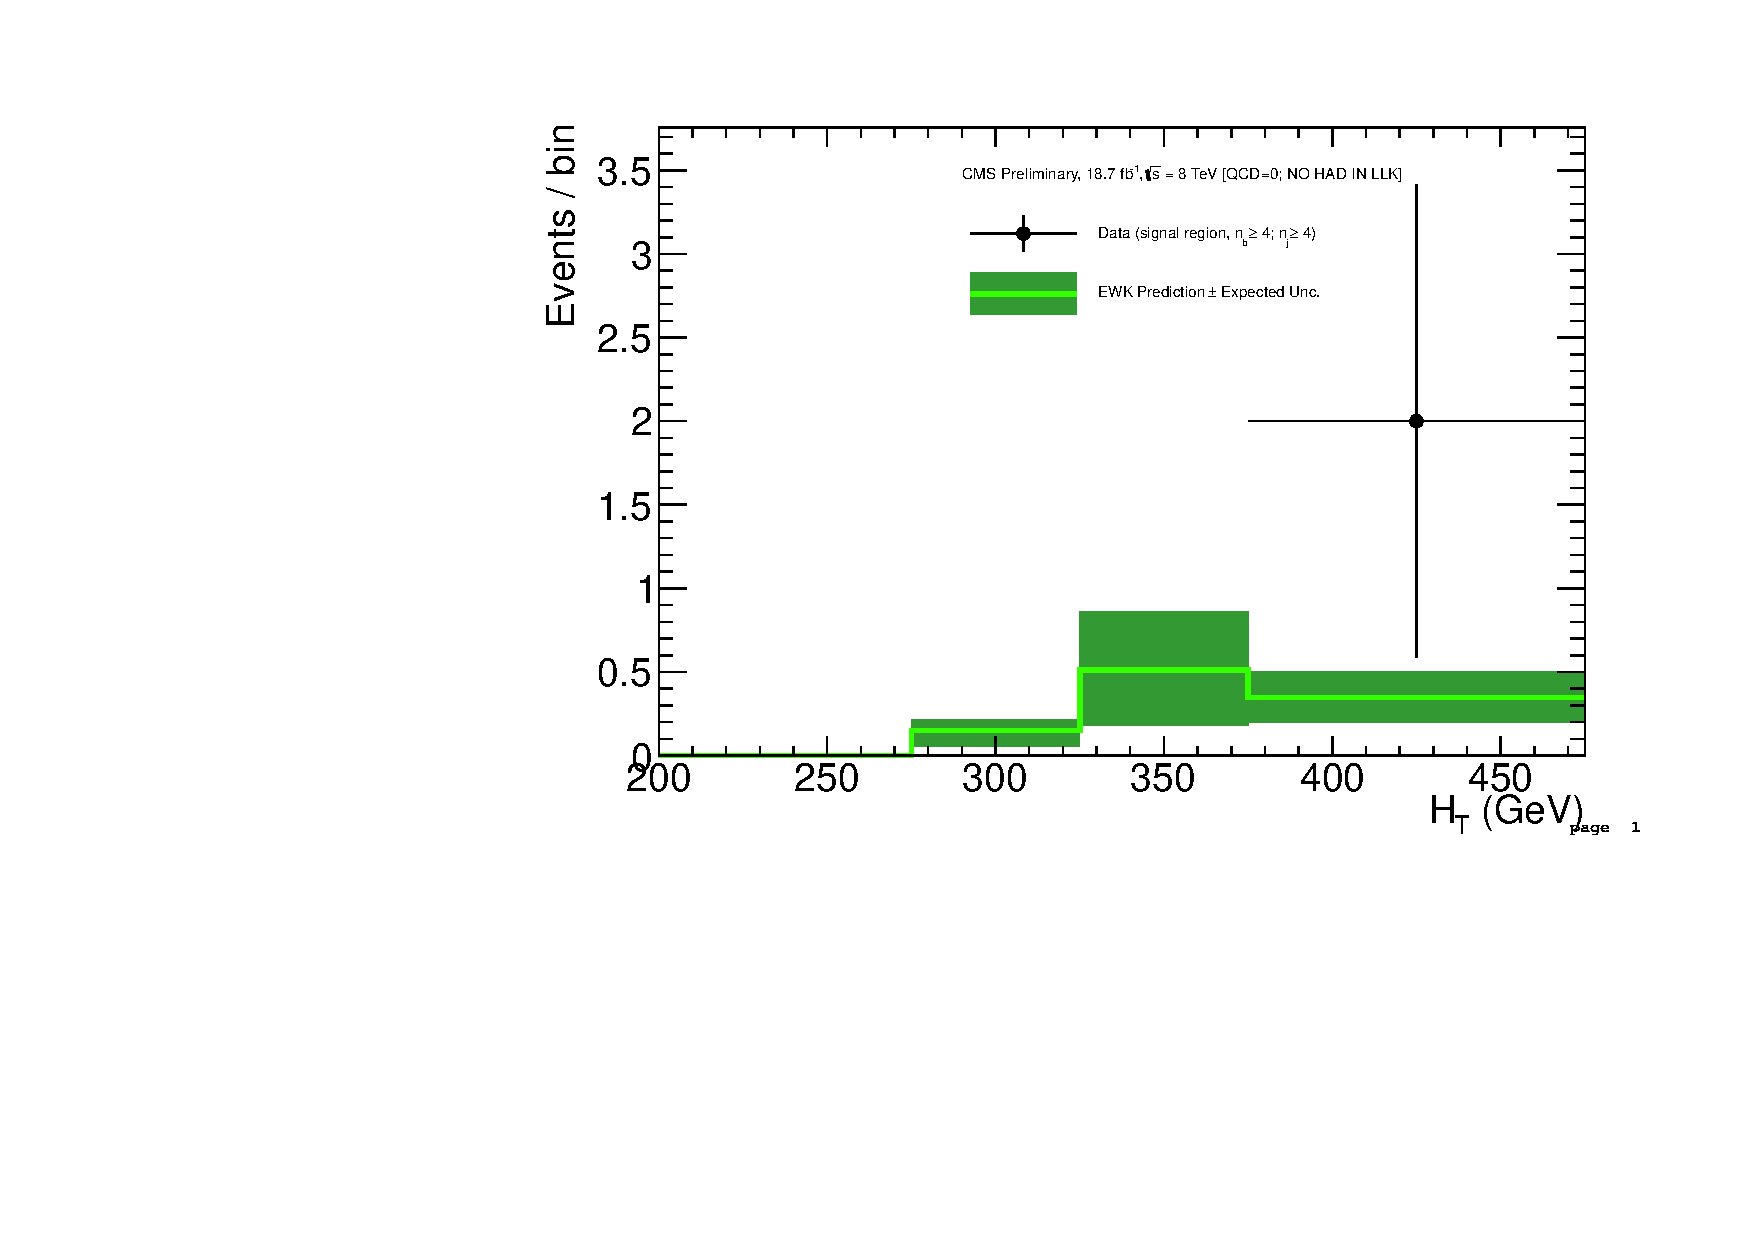
\includegraphics[width=\textwidth,page=1]
    {Figs/results/v0/greenBand/bestFit_2012dev_RQcdZero_fZinvAll_ge4b_ge4j-1_smOnly}
    \caption{Hadronic sample (linear scale)}
  \end{subfigure}
  \begin{subfigure}[b]{0.48\textwidth}
    \includegraphics[width=\textwidth,page=2]
    {Figs/results/v0/greenBand/bestFit_2012dev_RQcdZero_fZinvAll_ge4b_ge4j-1_smOnly}
    \caption{Hadronic sample (logarithmic scale)}
  \end{subfigure}
  \begin{subfigure}[b]{0.48\textwidth}
    \includegraphics[width=\textwidth,page=4]
    {Figs/results/v0/greenBand/bestFit_2012dev_RQcdZero_fZinvAll_ge4b_ge4j-1_smOnly}
    \caption{\mj sample}
  \end{subfigure}
  \caption{\njhigh, $\nb \geq 4$}
  \label{fig:green_fits_ge4b_ge4j}
\end{figure}

%%%%%%%%%%%%%%%%%%%%%%%%%%%%%%%%%%%
% BLUE BAND PLOTS
%%%%%%%%%%%%%%%%%%%%%%%%%%%%%%%%%%%

\clearpage
\begin{figure}[h!]
  \centering
  \begin{subfigure}[b]{0.48\textwidth}
    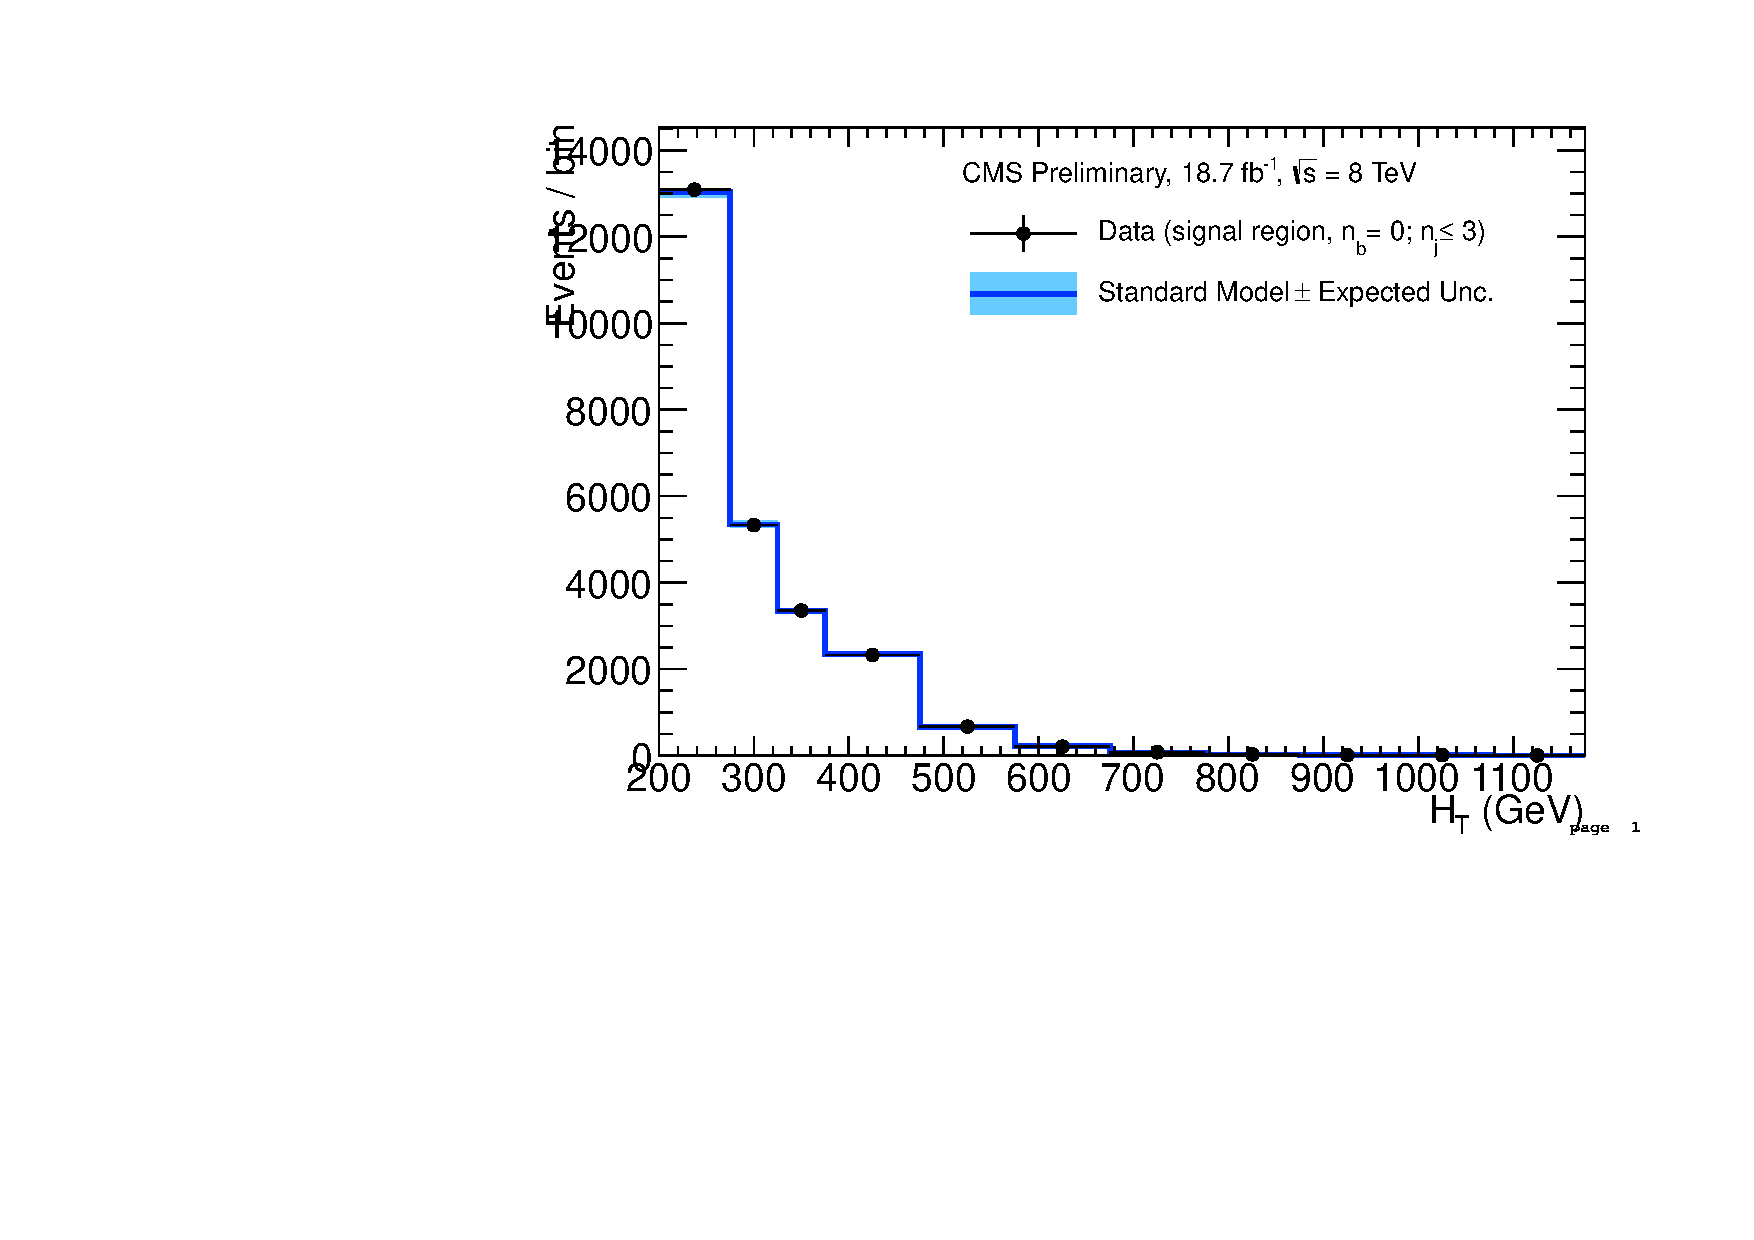
\includegraphics[width=\textwidth,page=1]
    {Figs/results/v0/blueBand/bestFit_2012dev_RQcdZero_fZinvAll_0b_le3j-12hp_smOnly}
    \caption{Hadronic sample (linear scale)}
  \end{subfigure}
  \begin{subfigure}[b]{0.48\textwidth}
    \includegraphics[width=\textwidth,page=2]
    {Figs/results/v0/blueBand/bestFit_2012dev_RQcdZero_fZinvAll_0b_le3j-12hp_smOnly}
    \caption{Hadronic sample (logarithmic scale)}
  \end{subfigure}
  \begin{subfigure}[b]{0.48\textwidth}
    \includegraphics[width=\textwidth,page=4]
    {Figs/results/v0/blueBand/bestFit_2012dev_RQcdZero_fZinvAll_0b_le3j-12hp_smOnly}
    \caption{\mj sample}
  \end{subfigure}
  \begin{subfigure}[b]{0.48\textwidth}
    \includegraphics[width=\textwidth,page=8]
    {Figs/results/v0/blueBand/bestFit_2012dev_RQcdZero_fZinvAll_0b_le3j-12hp_smOnly}
    \caption{\mmj sample}
  \end{subfigure}\\
  \begin{subfigure}[b]{0.48\textwidth}
    \includegraphics[width=\textwidth,page=6]
    {Figs/results/v0/blueBand/bestFit_2012dev_RQcdZero_fZinvAll_0b_le3j-12hp_smOnly}
    \caption{\gj sample}
  \end{subfigure}
  \caption{\njlow, $\nb = 0$}
  \label{fig:blue_fits_0b_le3j}
\end{figure}

\clearpage
\begin{figure}[h!]
  \centering
  \begin{subfigure}[b]{0.48\textwidth}
    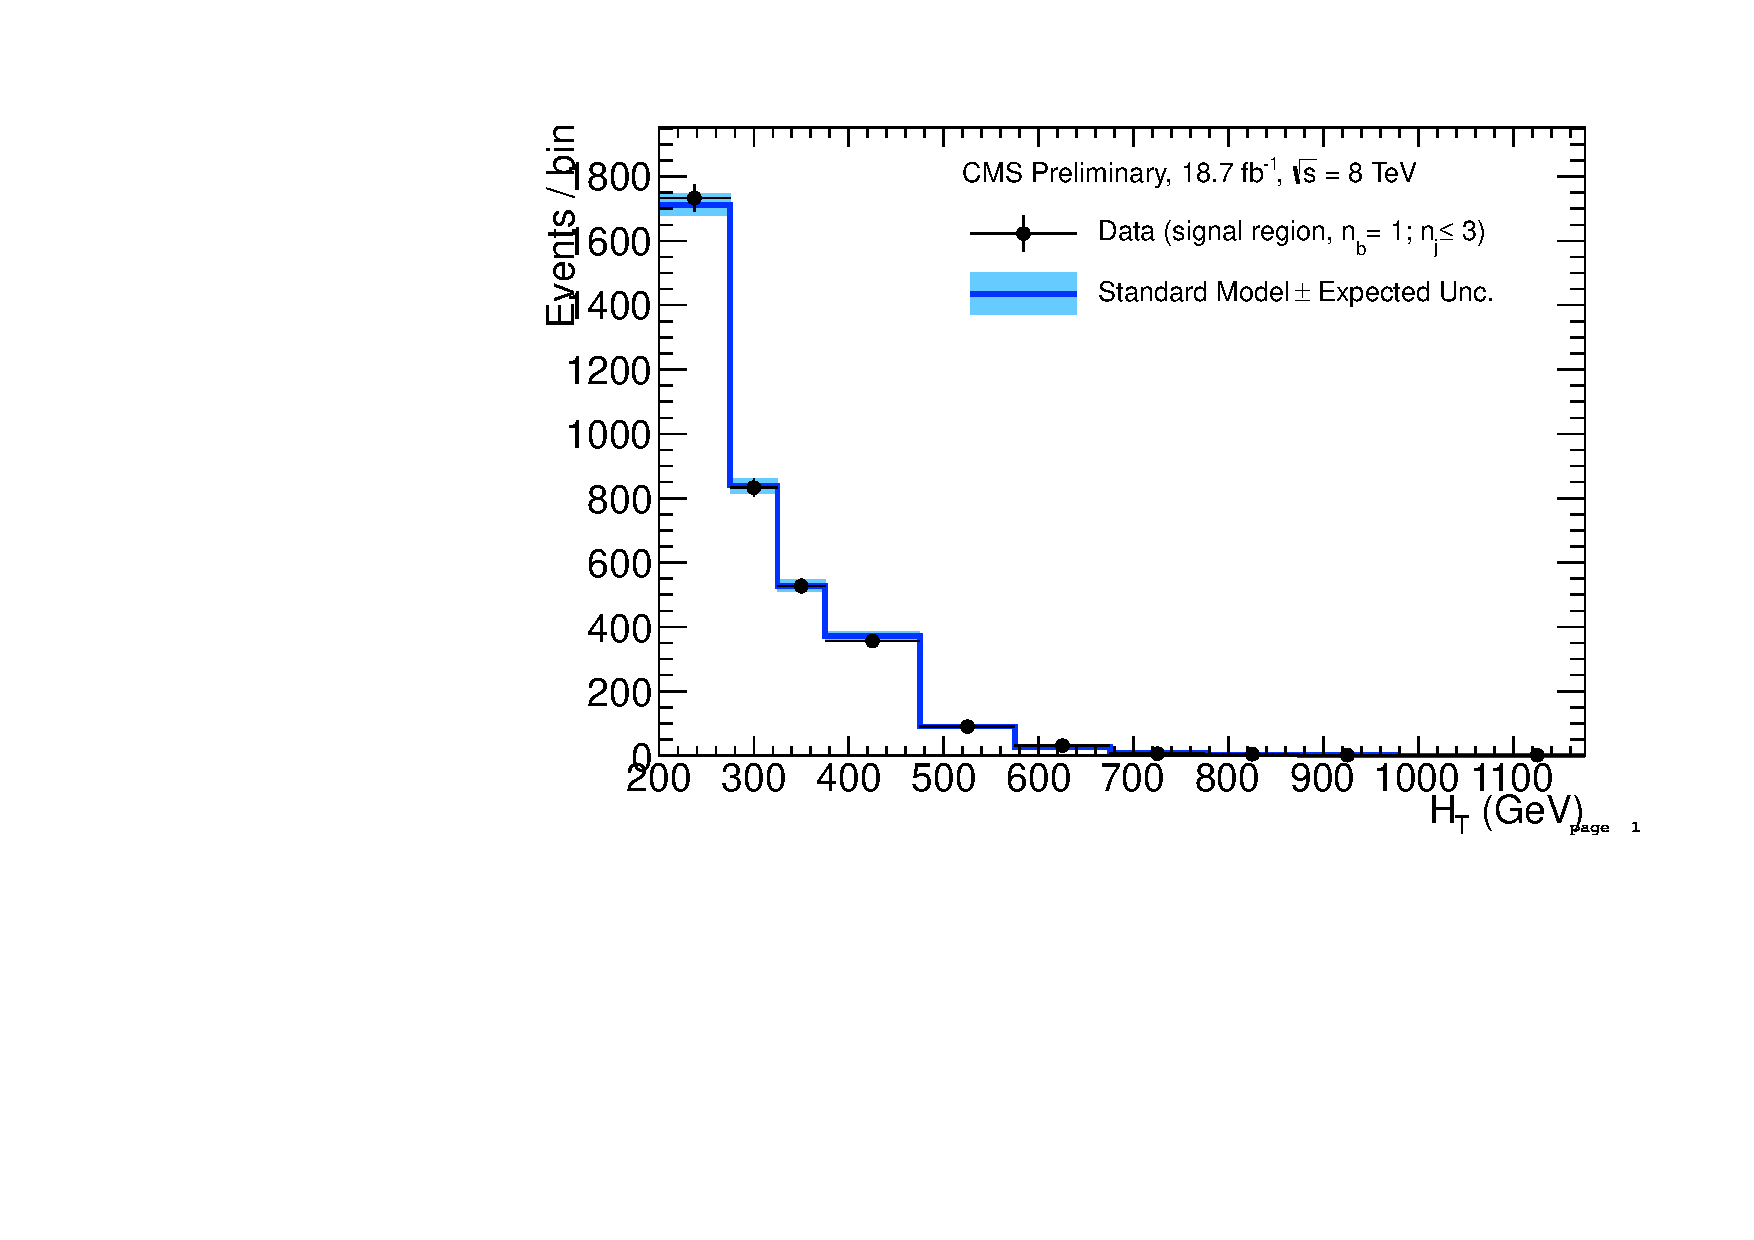
\includegraphics[width=\textwidth,page=1]
    {Figs/results/v0/blueBand/bestFit_2012dev_RQcdZero_fZinvAll_1b_le3j-12hp_smOnly}
    \caption{Hadronic sample (linear scale)}
  \end{subfigure}
  \begin{subfigure}[b]{0.48\textwidth}
    \includegraphics[width=\textwidth,page=2]
    {Figs/results/v0/blueBand/bestFit_2012dev_RQcdZero_fZinvAll_1b_le3j-12hp_smOnly}
    \caption{Hadronic sample (logarithmic scale)}
  \end{subfigure}
  \begin{subfigure}[b]{0.48\textwidth}
    \includegraphics[width=\textwidth,page=4]
    {Figs/results/v0/blueBand/bestFit_2012dev_RQcdZero_fZinvAll_1b_le3j-12hp_smOnly}
    \caption{\mj sample}
  \end{subfigure}
  \begin{subfigure}[b]{0.48\textwidth}
    \includegraphics[width=\textwidth,page=8]
    {Figs/results/v0/blueBand/bestFit_2012dev_RQcdZero_fZinvAll_1b_le3j-12hp_smOnly}
    \caption{\mmj sample}
  \end{subfigure}\\
  \begin{subfigure}[b]{0.48\textwidth}
    \includegraphics[width=\textwidth,page=6]
    {Figs/results/v0/blueBand/bestFit_2012dev_RQcdZero_fZinvAll_1b_le3j-12hp_smOnly}
    \caption{\gj sample}
  \end{subfigure}
  \caption{\njlow, $\nb = 1$}
  \label{fig:blue_fits_1b_le3j}
\end{figure}

\clearpage
\begin{figure}[h!]
  \centering
  \begin{subfigure}[b]{0.48\textwidth}
    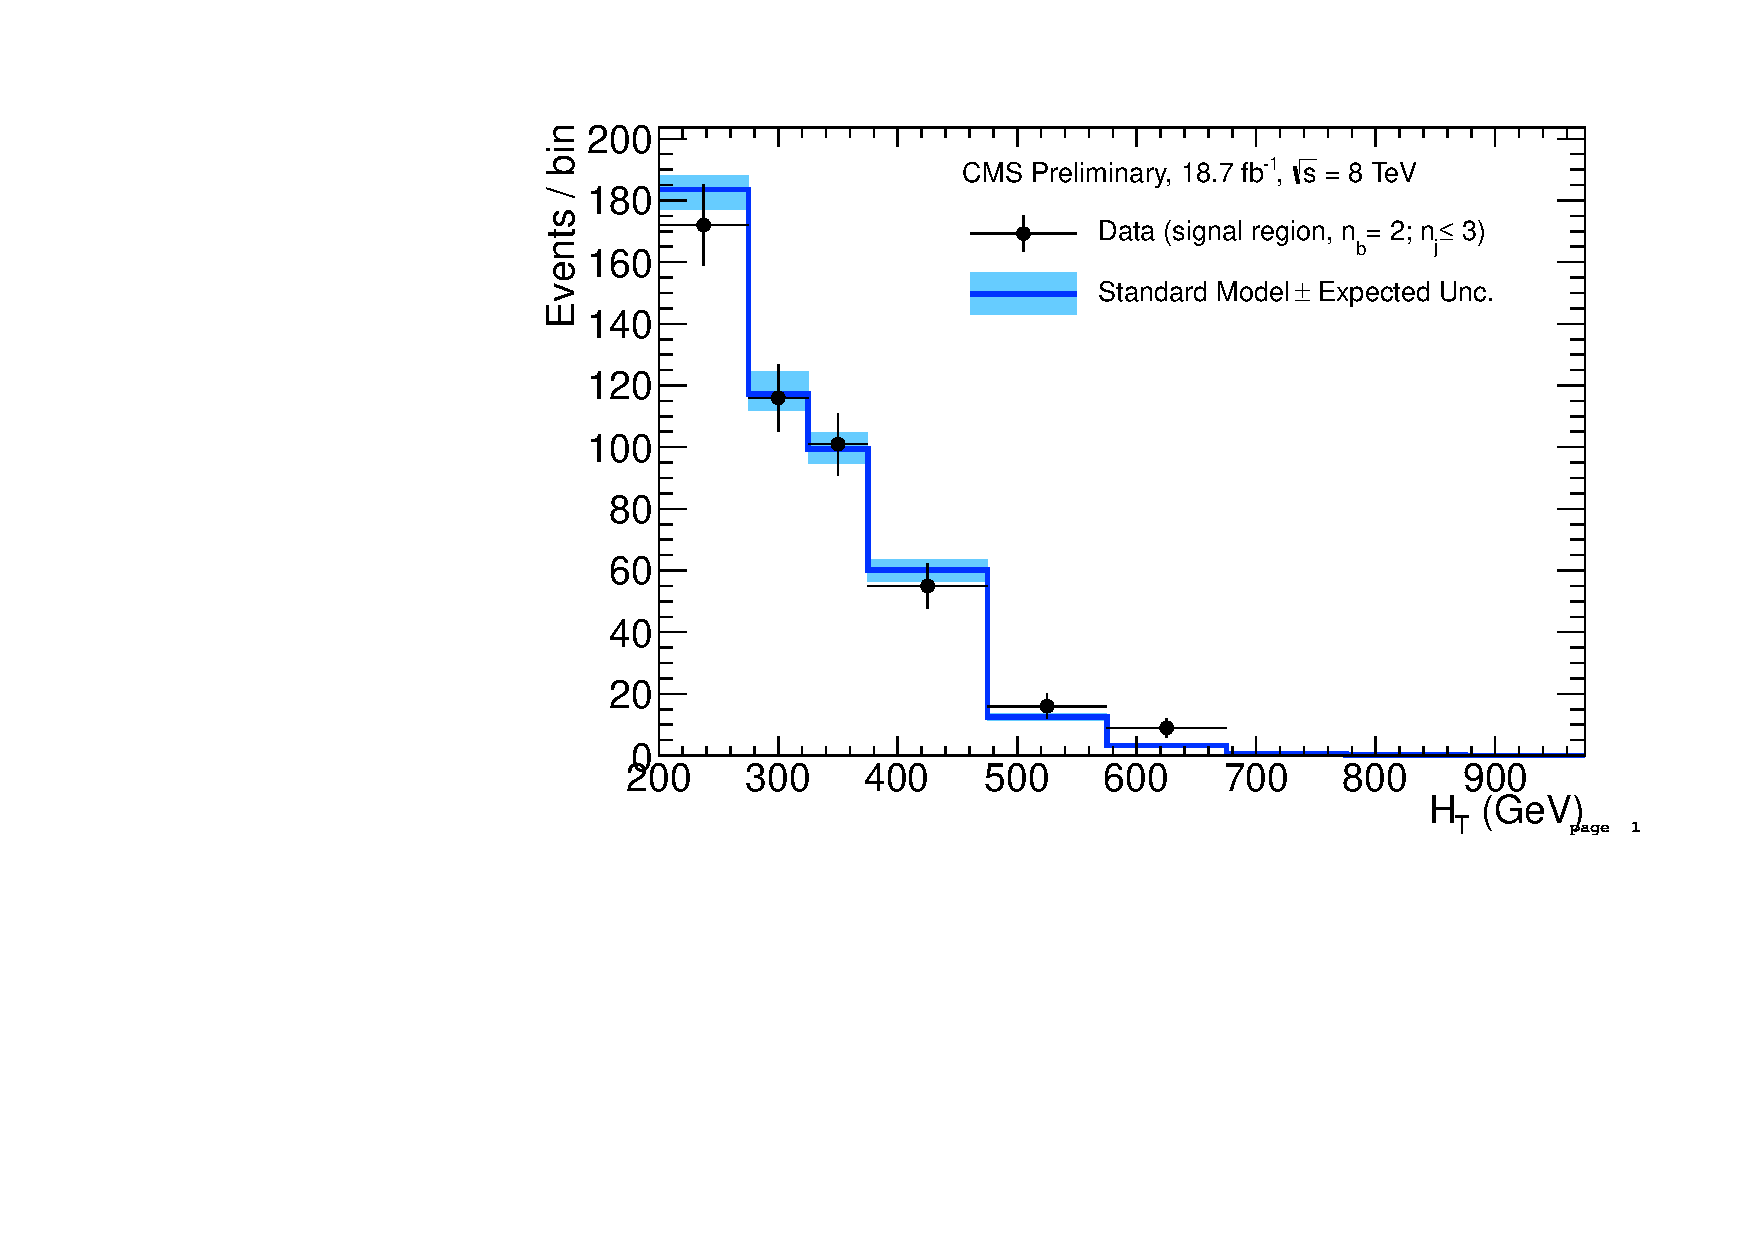
\includegraphics[width=\textwidth,page=1]
    {Figs/results/v0/blueBand/bestFit_2012dev_RQcdZero_fZinvAll_2b_le3j-1h_smOnly}
    \caption{Hadronic sample (linear scale)}
  \end{subfigure}
  \begin{subfigure}[b]{0.48\textwidth}
    \includegraphics[width=\textwidth,page=2]
    {Figs/results/v0/blueBand/bestFit_2012dev_RQcdZero_fZinvAll_2b_le3j-1h_smOnly}
    \caption{Hadronic sample (logarithmic scale)}
  \end{subfigure}
  \begin{subfigure}[b]{0.48\textwidth}
    \includegraphics[width=\textwidth,page=4]
    {Figs/results/v0/blueBand/bestFit_2012dev_RQcdZero_fZinvAll_2b_le3j-1h_smOnly}
    \caption{\mj sample}
  \end{subfigure}
  \caption{\njlow, $\nb = 2$}
  \label{fig:blue_fits_2b_le3j}
\end{figure}

\clearpage
\begin{figure}[h!]
  \centering
  \begin{subfigure}[b]{0.48\textwidth}
    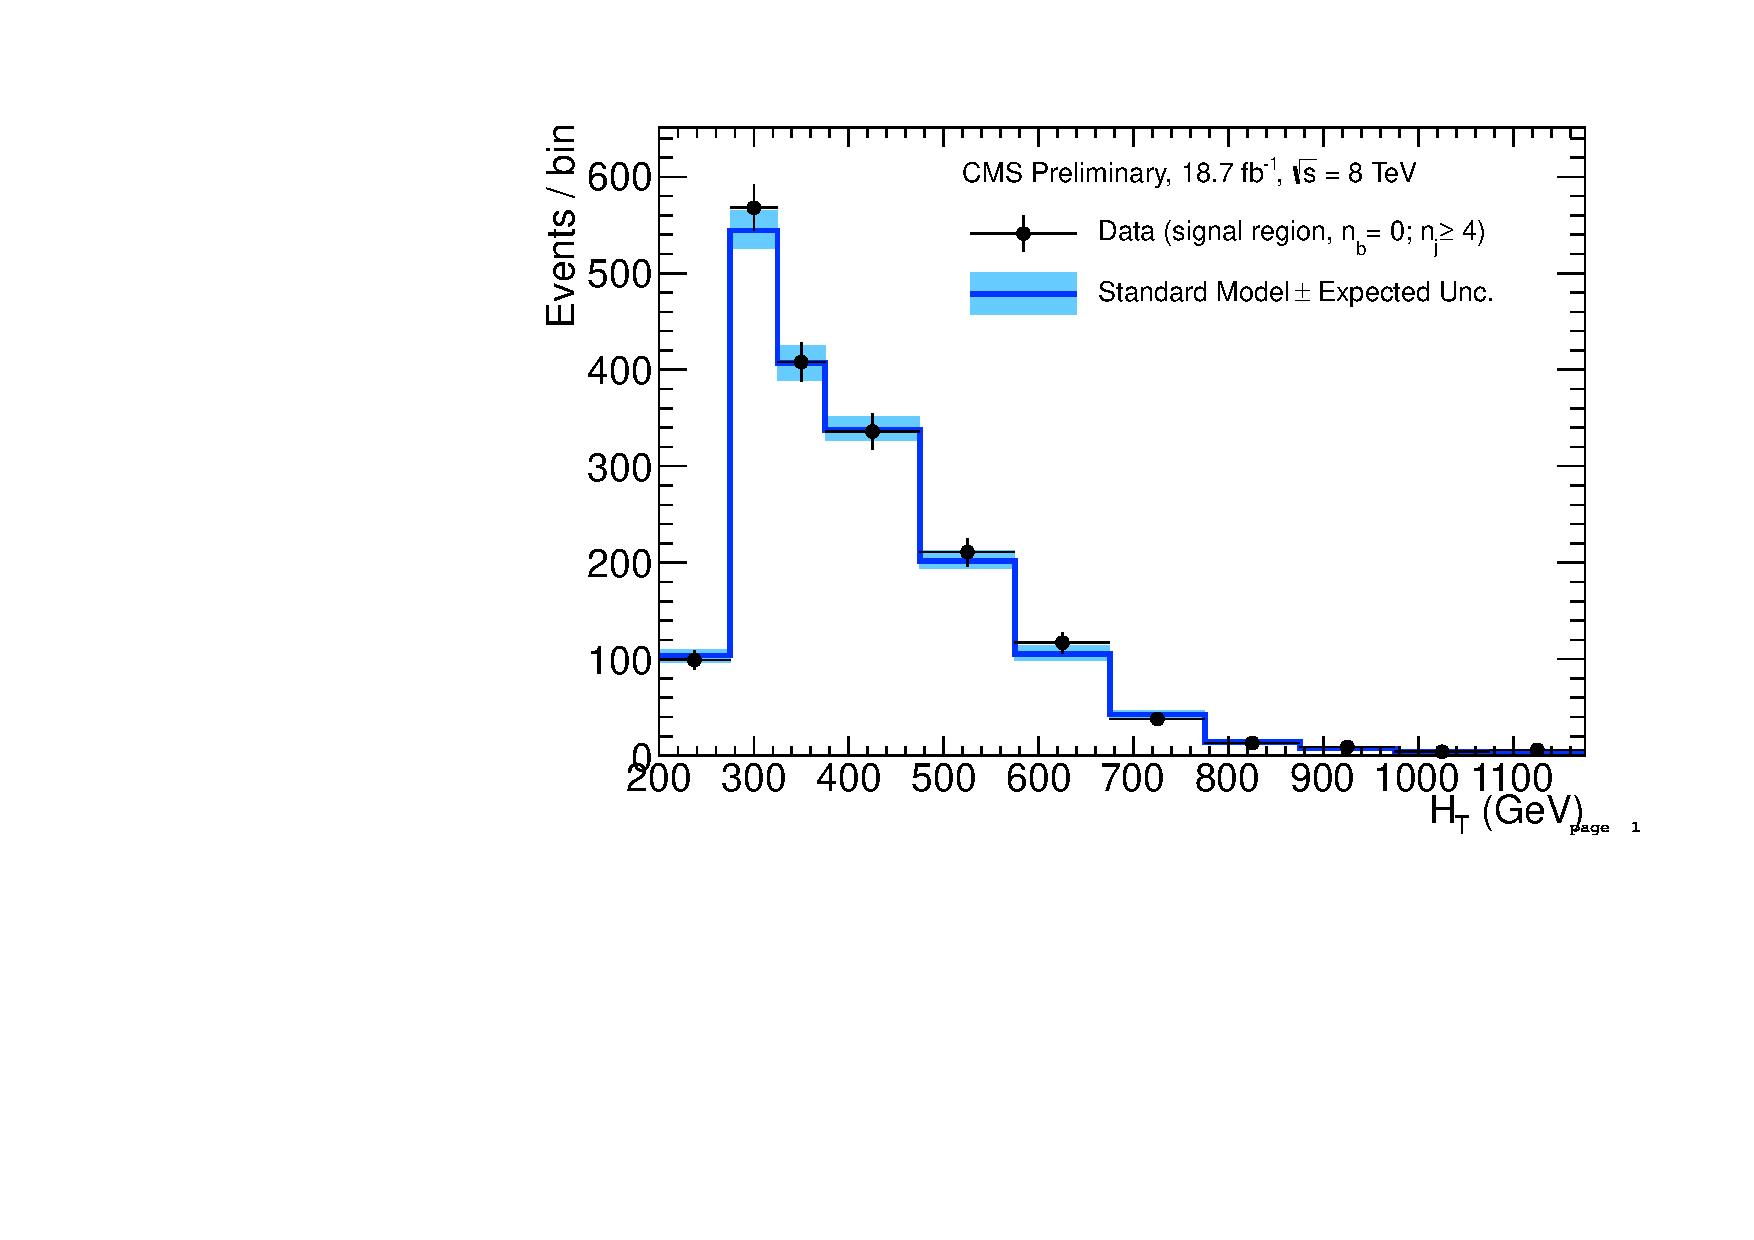
\includegraphics[width=\textwidth,page=1]
    {Figs/results/v0/blueBand/bestFit_2012dev_RQcdZero_fZinvAll_0b_ge4j-12hp_smOnly}
    \caption{Hadronic sample (linear scale)}
  \end{subfigure}
  \begin{subfigure}[b]{0.48\textwidth}
    \includegraphics[width=\textwidth,page=2]
    {Figs/results/v0/blueBand/bestFit_2012dev_RQcdZero_fZinvAll_0b_ge4j-12hp_smOnly}
    \caption{Hadronic sample (logarithmic scale)}
  \end{subfigure}
  \begin{subfigure}[b]{0.48\textwidth}
    \includegraphics[width=\textwidth,page=4]
    {Figs/results/v0/blueBand/bestFit_2012dev_RQcdZero_fZinvAll_0b_ge4j-12hp_smOnly}
    \caption{\mj sample}
  \end{subfigure}
  \begin{subfigure}[b]{0.48\textwidth}
    \includegraphics[width=\textwidth,page=8]
    {Figs/results/v0/blueBand/bestFit_2012dev_RQcdZero_fZinvAll_0b_ge4j-12hp_smOnly}
    \caption{\mmj sample}
  \end{subfigure}\\
  \begin{subfigure}[b]{0.48\textwidth}
    \includegraphics[width=\textwidth,page=6]
    {Figs/results/v0/blueBand/bestFit_2012dev_RQcdZero_fZinvAll_0b_ge4j-12hp_smOnly}
    \caption{\gj sample}
  \end{subfigure}
  \caption{\njhigh, $\nb = 0$}
  \label{fig:blue_fits_0b_ge4j}
\end{figure}

\clearpage
\begin{figure}[h!]
  \centering
  \begin{subfigure}[b]{0.48\textwidth}
    \includegraphics[width=\textwidth,page=1]
    {Figs/results/v0/blueBand/bestFit_2012dev_RQcdZero_fZinvAll_1b_ge4j-12hp_smOnly}
    \caption{Hadronic sample (linear scale)}
  \end{subfigure}
  \begin{subfigure}[b]{0.48\textwidth}
    \includegraphics[width=\textwidth,page=2]
    {Figs/results/v0/blueBand/bestFit_2012dev_RQcdZero_fZinvAll_1b_ge4j-12hp_smOnly}
    \caption{Hadronic sample (logarithmic scale)}
  \end{subfigure}
  \begin{subfigure}[b]{0.48\textwidth}
    \includegraphics[width=\textwidth,page=4]
    {Figs/results/v0/blueBand/bestFit_2012dev_RQcdZero_fZinvAll_1b_ge4j-12hp_smOnly}
    \caption{\mj sample}
  \end{subfigure}
  \begin{subfigure}[b]{0.48\textwidth}
    \includegraphics[width=\textwidth,page=8]
    {Figs/results/v0/blueBand/bestFit_2012dev_RQcdZero_fZinvAll_1b_ge4j-12hp_smOnly}
    \caption{\mmj sample}
  \end{subfigure}\\
  \begin{subfigure}[b]{0.48\textwidth}
    \includegraphics[width=\textwidth,page=6]
    {Figs/results/v0/blueBand/bestFit_2012dev_RQcdZero_fZinvAll_1b_ge4j-12hp_smOnly}
    \caption{\gj sample}
  \end{subfigure}
  \caption{\njhigh, $\nb = 1$}
  \label{fig:blue_fits_1b_ge4j}
\end{figure}

\clearpage
\begin{figure}[h!]
  \centering
  \begin{subfigure}[b]{0.48\textwidth}
    \includegraphics[width=\textwidth,page=1]
    {Figs/results/v0/blueBand/bestFit_2012dev_RQcdZero_fZinvAll_2b_ge4j-1h_smOnly}
    \caption{Hadronic sample (linear scale)}
  \end{subfigure}
  \begin{subfigure}[b]{0.48\textwidth}
    \includegraphics[width=\textwidth,page=2]
    {Figs/results/v0/blueBand/bestFit_2012dev_RQcdZero_fZinvAll_2b_ge4j-1h_smOnly}
    \caption{Hadronic sample (logarithmic scale)}
  \end{subfigure}
  \begin{subfigure}[b]{0.48\textwidth}
    \includegraphics[width=\textwidth,page=4]
    {Figs/results/v0/blueBand/bestFit_2012dev_RQcdZero_fZinvAll_2b_ge4j-1h_smOnly}
    \caption{\mj sample}
  \end{subfigure}
  \caption{\njhigh, $\nb = 2$}
  \label{fig:blue_fits_2b_ge4j}
\end{figure}


\clearpage
\begin{figure}[h!]
  \centering
  \begin{subfigure}[b]{0.48\textwidth}
    \includegraphics[width=\textwidth,page=1]
    {Figs/results/v0/blueBand/bestFit_2012dev_RQcdZero_fZinvAll_3b_ge4j-1h_smOnly}
    \caption{Hadronic sample (linear scale)}
  \end{subfigure}
  \begin{subfigure}[b]{0.48\textwidth}
    \includegraphics[width=\textwidth,page=2]
    {Figs/results/v0/blueBand/bestFit_2012dev_RQcdZero_fZinvAll_3b_ge4j-1h_smOnly}
    \caption{Hadronic sample (logarithmic scale)}
  \end{subfigure}
  \begin{subfigure}[b]{0.48\textwidth}
    \includegraphics[width=\textwidth,page=4]
    {Figs/results/v0/blueBand/bestFit_2012dev_RQcdZero_fZinvAll_3b_ge4j-1h_smOnly}
    \caption{\mj sample}
  \end{subfigure}
  \caption{\njhigh, $\nb = 3$}
  \label{fig:blue_fits_3b_ge4j}
\end{figure}

\clearpage
\begin{figure}[h!]
  \centering
  \begin{subfigure}[b]{0.48\textwidth}
    \includegraphics[width=\textwidth,page=1]
    {Figs/results/v0/blueBand/bestFit_2012dev_RQcdZero_fZinvAll_ge4b_ge4j-1h_smOnly}
    \caption{Hadronic sample (linear scale)}
  \end{subfigure}
  \begin{subfigure}[b]{0.48\textwidth}
    \includegraphics[width=\textwidth,page=2]
    {Figs/results/v0/blueBand/bestFit_2012dev_RQcdZero_fZinvAll_ge4b_ge4j-1h_smOnly}
    \caption{Hadronic sample (logarithmic scale)}
  \end{subfigure}
  \begin{subfigure}[b]{0.48\textwidth}
    \includegraphics[width=\textwidth,page=4]
    {Figs/results/v0/blueBand/bestFit_2012dev_RQcdZero_fZinvAll_ge4b_ge4j-1h_smOnly}
    \caption{\mj sample}
  \end{subfigure}
  \caption{\njhigh, $\nb \geq 4$}
  \label{fig:blue_fits_ge4b_ge4j}
\end{figure}
